	%%%%%%%%%%%%%%%%%%%%%%%%%%%%%%%%%%%%%%%%%%%%%%%%%%%%%%%%%%%%%%%%%%%%%%%%
% 
% LaTeX Template
%
%%%%%%%%%%%%%%%%%%%%%%%%%%%%%%%%%%%%%%%%%%%%%%%%%%%%%%%%%%%%%%%%%%%%%%%%

%------------------------------------------------------------------------------------------------
%	DOCUMENT CONFIGURATIONS
%------------------------------------------------------------------------------------------------

% DOCUMENT
%   - Properties
\documentclass[a4paper,11pt]{report} % Sets a two-sided A4 sized paper.
                                         % (Two-sided for LaTeX to distinguish between odd/even
                                         % pages while using headers and footers.)
\linespread{1.15}                         % Default space between lines
                                    % Margin sizes defined in headers_and_footers file.
\usepackage[nottoc,numbib]{tocbibind}    % Makes References section appear in the Table of contents (nottoc). Conuts the References like section.
\usepackage{lastpage}                    % To get the total number of pages.

%   - Sectioning
\usepackage{titlesec}                   % Extra features for sectioning
    % The following lines create: \subsubsubsection{}
    
    
%%%%%%%%% From here: creation of \subsubsubsection{} %%%%%%%%%
    \titleclass{\subsubsubsection}{straight}[\subsection]

    \newcounter{subsubsubsection}[subsubsection]
    \renewcommand\thesubsubsubsection{\thesubsubsection.\arabic{subsubsubsection}}
    \renewcommand\theparagraph{\thesubsubsubsection.\arabic{paragraph}} % optional; useful if paragraphs are to be numbered

    \titleformat{\subsubsubsection}
      {\normalfont\normalsize\bfseries}{\thesubsubsubsection}{1em}{}
    \titlespacing*{\subsubsubsection}
    {0pt}{3.25ex plus 1ex minus .2ex}{1.5ex plus .2ex}

    \makeatletter
    \renewcommand\paragraph{\@startsection{paragraph}{5}{\z@}%
      {3.25ex \@plus1ex \@minus.2ex}%
      {-1em}%
      {\normalfont\normalsize\bfseries}}
    \renewcommand\subparagraph{\@startsection{subparagraph}{6}{\parindent}%
      {3.25ex \@plus1ex \@minus .2ex}%
      {-1em}%
      {\normalfont\normalsize\bfseries}}
    \def\toclevel@subsubsubsection{4}
    \def\toclevel@paragraph{5}
    \def\toclevel@paragraph{6}
    \def\l@subsubsubsection{\@dottedtocline{4}{7em}{4em}}
    \def\l@paragraph{\@dottedtocline{5}{10em}{5em}}
    \def\l@subparagraph{\@dottedtocline{6}{14em}{6em}}
    \makeatother

    \setcounter{secnumdepth}{4}
    \setcounter{tocdepth}{4}
%%%%%%%%% Until here: creation of \subsubsubsection{} %%%%%%%%%


%\let\oldsection\section % This line and the following force sections to start on odd pages.
%\def\section{\cleardoublepage\oldsection}

\newcommand*{\blankpage}{%
    \vspace*{\fill}
        \begin{center}
            (This page was intentionally left in blank.)
        \end{center}
    \vspace{\fill}
}
\makeatletter
\renewcommand*{\cleardoublepage}{\clearpage\if@twoside \ifodd\c@page\else
\blankpage
\thispagestyle{empty}
\newpage
\if@twocolumn\hbox{}\newpage\fi\fi\fi}
\makeatother

% WRITING
%   - Math/Chemistry/...
\usepackage{amsmath}                % Mathematical features.
    % Section numbering
    \numberwithin{equation}{section}    % Equation numbering by section
    \numberwithin{table}{section}       % Table numbering by section
    \numberwithin{figure}{section}      % Table numbering by section
\usepackage{amssymb}                % Symbols.
\usepackage[version=3]{mhchem}                 % Chemical equation typesetting. i.e.: \ce{CO2 + C <=> 2CO}
\usepackage{siunitx}                % Simplifies the usage of values with units.
                                    % i.e.: "\SI{5.4}{kg·m^{-1}·s^{-2}}"
                                    % instead of "5.4 kg·m$ ^{-1} $·s$ ^{-2} $"
\usepackage{eurosym}                % Use EURO symbol (\euro)

%%   - Language
\usepackage[utf8]{inputenc}         % Required for the usage of characters like 'ñ', 'ú', ...
%\renewcommand{\figurename}{Figura}  % In captions, print "Figura" (in Catalan) instead of
                                    % "Figure" (English default name).
%\renewcommand{\tablename}{Tabla}
%\renewcommand{\contentsname}{Índice}
%\renewcommand{\refname}{Bibliografía}

%   - Text
%\let\oldsection\section             % This line and the nextone force sections to start always in new odd pages.
%\def\section{\cleardoublepage\oldsection} %
\usepackage[none]{hyphenat}         % [none] Prevents any hyphenation throughout the document.
                                    % (hyphenation -> "separació per síl·labes")
\sloppy                             % Forces wrapping at word boundaries by relaxing the interword space constraints.
%\usepackage{indentfirst}            % Forces indentation from paragraphs after a section.
                                    % (see notes 1 and 2)
\setlength\parindent{1cm}           % Removes all indentation from paragraphs.
%\newenvironment{paragraphs}{\setlength\parindent{1cm}}{\setlength\parindent{0cm}}
                                    % "\begin{paragraphs}" will create an environment where
                                    % indentation from paragraphs is activated.
\usepackage[font=footnotesize]{caption} % Captions
\setlength{\abovecaptionskip}{0pt}      %
\setlength{\belowcaptionskip}{0pt}      %
\usepackage{lmodern}                % Allow the use of font size larger tha 25pt
\usepackage[T1]{fontenc}            %

% GRAPHICS, TABLES AND OTHERS
\usepackage{graphicx}               % Required for the inclusion of images.
\usepackage{float}                  % Required for some float properties.
\usepackage{pdfpages}               % Required for the inclusion of PDF files.
\usepackage{multirow,longtable,array,booktabs,tabularx} % More features for tables.
\usepackage{enumerate}              % Gives the enumerate environment an optional argument which
                                    % determines the style in which the counter is printed.
\usepackage{enumitem}               % Extra options for "enumerate" lists
\usepackage{color}                  % Use some color options.
\usepackage{colortbl}               % Use some other color options.
	\definecolor{UPC_blue}{RGB}{67,142,197}
	\definecolor{lightgrey}{RGB}{166,166,166}
\usepackage{hyperref}               % Provides LeTeX the hability to create hyperlinks.

\usepackage{inputenc}         % It makes possible to use roman numbers for the pages before the first chapter and arabic for the rest of the document

\usepackage{booktabs}
\usepackage{xcolor,colortbl}
\usepackage{pstricks}
\usepackage{blindtext}
\usepackage{transparent}
\usepackage{etoolbox}
\usepackage{pdflscape}
\usepackage{amsmath}
\usepackage{amsfonts}
\usepackage{amssymb}
\usepackage{graphicx}
\usepackage{eurosym}
\usepackage{wrapfig}
\usepackage{mathdots}
\usepackage{caption}
\usepackage{cite}
\usepackage{mathrsfs}
\usepackage{float}
\usepackage{import}
\usepackage{makecell}
\usepackage{booktabs}
\usepackage{graphicx}

%   - NOTES
% (1) LaTeX implements a style that doesn't indent the first paragraph after a section heading. There are coherent reasons for this. Some typography rules state that first indent should be suppressed only after a centered title and that all other paragraphs must be indented.
% (2) We have already removed all indentation from paragraphs with the command "\setlength\parindent{0cm}", but when using the environment we've created "escrit" we set indent to 1cm. Then, if this environment is used right after a section the first indent will be suppressed unless we use the package "indentfirst". % Document Configurations

%-----------------------------------------------------------------------------
%	REPORT INFORMATION
%-----------------------------------------------------------------------------

%%% MAIN INFORMATION %%%

% School
\newcommand{\School}{ESEIAAT}
\newcommand{\researcherDept}{UPC - HIRO}
% Degree
\newcommand{\Degree}{Aerospace Technology Engineering}

% Department
\newcommand{\Department}{UPC Departament d'Enginyeria de Projectes i de la Construcció}

% Secció (Secció de Terrassa)
\newcommand{\Seccio}{Secció de Terrassa}

% Course
\newcommand{\Course}{Degree Final Project}

% Group
\newcommand{\Group}{G3-PM-P2018}

% Students (if you don't use that much students, leave them in blank)
\newcommand{\Studi}	    {Calderón Rosario, Borja}
\newcommand{\Studii}	{De Benedicto Barba, Maria}
\newcommand{\Studiii}	{Escartín Vivancos, Guillermo}
\newcommand{\Studiv}	{Fontanes Molina, Pol}
\newcommand{\Studv}	    {Franch I Ruiz, Sergi}
\newcommand{\Studvi}	{González García, Sílvia}
\newcommand{\Studvii}	{Herrando Moraira, Albert}
\newcommand{\Studviii}	{Lopezbarrena Arenas, Santiago}
\newcommand{\Studix}	{Nachett, Hamza}
\newcommand{\Studx}	    {Pérez Sánchez, David}
\newcommand{\Studxi}	{Pla Olea, Laura}
\newcommand{\Studxii}	{Pons Daza, Marina}
\newcommand{\Studxiii}	{Ramón Costa, Fernando}
\newcommand{\Studxiv}	{Sellart Combalia, Ana Maria}
\newcommand{\Studxv}	{Serra Moncunill, Josep Maria}
\newcommand{\Studxvi}	{Urbano González, Eva María}


% Customer:
\newcommand{\Director}{Pérez Llera, Luís Manuel}
\newcommand{\CoDirector}{Williams, Earle}

% Project Name
\newcommand{\ProjectName}{Project DEOS-UD}
\newcommand{\ProjectsubName}{Disruptive Earth Observation Sensing for Urban Developement}
% Acronym
\newcommand{\Acronym}{HIRO}

% Short Name
\newcommand{\ShortName}{HIRO}

% Kind of document
\newcommand{\DocTypeI}{Deliverable 1}
\newcommand{\DocTypeII}{Project Charter}

% Page number preceding (leave in blank if nothing is required)
% Suggestion: R, RA, B, D, T referred to report, report attachments, budget, drawings or technical sheets
\newcommand{\precPage}{PC}


% Date of the document (Delivery date)
	% Day
	\newcommand{\DocDateD}{16}
	% Month
	\newcommand{\DocDateM}{03}
	% Year
	\newcommand{\DocDateY}{2018}

%-----------------------------------------------------------------------------
% Don't touch this unless you know what you are doing!

% Generation of Group Code
\newcommand{\GrCode}{{\GrNum} EA-\GrTerm\GrYr} 

% Generation of the date format
\newcommand{\DocDate}{\DocDateD-\DocDateM-\DocDateY}  % Document information

%-----------------------------------------------------------------------------
%	HEADERS AND FOOTERS
%-----------------------------------------------------------------------------

% Changes default margins.
\usepackage[left=3cm,right=3cm,top=2.5cm,bottom=2.5cm]{geometry}
   \setlength{\headheight}{50pt}         % Header Space.
   \setlength{\textheight}{640pt}        % Text height.
   \setlength{\footskip}{30pt}           % Foot Space.

\usepackage{fancyhdr}
	\pagestyle{fancy} % Headers and footers -> "fancy" style.
	
	% Obtain the name of the section:
	\renewcommand{\sectionmark}[1]{\markright{Section \thesection : #1}}
	\renewcommand{\chaptermark}[1]{\markleft{Chapter \thechapter : #1}} 

	\fancyhf{} % Clear all headers and footers fields

% Package info and examples
%		% O/E = Odd/Even page // L/C/R = Left/Center/Right field
%	\fancyhead[LE]{\hspace{-10pt}
%		\raisebox{-\height+12pt}{
%		
\includegraphics[height=30pt]{./doc_config/images/UPC_dpt}
%		}
%	}
%	\fancyhead[RE]{\bf \Department}
%	\fancyhead[LO]{\bf \DocType}
%	\fancyhead[RO]{\bf \emph{\ProjectName}}
%	\fancyfoot[LE,RO]{\thepage} % Adds customized pages numbers



%-----------------------------------------------
% General headers and footers of the document:
%-----------------------------------------------
	% Headers
	\fancyhead[LO]{\textbf{\rightmark}} % Section mark
	\fancyhead[RO]{
\includegraphics[height=25pt]{./doc_config/images/logo3}}
	\fancyhead[LE]{\textbf{\rightmark}}
	\fancyhead[RE]{
\includegraphics[height=25pt]{./doc_config/images/logo3}}

	% Footers
	\fancyfoot[CE,CO]{\precPage{} - \thepage}
	\fancyfoot[LO,RE]{\textbf{\Acronym}}

	\renewcommand{\headrulewidth}{0.5pt} % Header decorative line
	\renewcommand{\footrulewidth}{0.5pt} % Footer decorative line
	\renewcommand{\chaptermark}[1]{%
\markboth{#1}{}}
\renewcommand{\sectionmark}[1]{\markright{#1}}


%-----------------------------------------------
% Headers and footers for pages where chapter starts:
%-----------------------------------------------
\fancypagestyle{plain}{
	%Headers
	\fancyhead[LO]{\textbf{\leftmark}} % Section mark
	\fancyhead[RO]{
\includegraphics[height=25pt]{./doc_config/images/logo3}}
	\fancyhead[LE]{\textbf{\leftmark}}
	\fancyhead[RE]{
\includegraphics[height=25pt]{./doc_config/images/logo3}}
	%Footers
	\fancyfoot[CE]{\precPage{} - \thepage}
	\fancyfoot[CO]{\precPage{} - \thepage}
	\fancyfoot[LO,RE]{\textbf{\Acronym}}
	
	\renewcommand{\headrulewidth}{0.5pt} % Header decorative line
	\renewcommand{\footrulewidth}{0.5pt} % Footer decorative line
}


%-----------------------------------------------
% Cover headers and footers:
%-----------------------------------------------

	\fancypagestyle{CoverPage}{ % This creates a new headers and footers page style.
	                            % To use it type "\thispagestyle{FirstPage}" on the first page.
	                                % (right after "\maketitle")
		\fancyhf{}
		%\fancyfoot[C]{Group \GrCode \hfill [\DocDate]}
		\renewcommand{\headrulewidth}{0pt}
		\renewcommand{\footrulewidth}{0pt}
	}


%-----------------------------------------------
% No headers nor footers page (ie: Back cover)
%-----------------------------------------------

	\fancypagestyle{EmptyPage}{
		\fancyhf{}
		\renewcommand{\headrulewidth}{0pt}
		\renewcommand{\footrulewidth}{0pt}
	} % Headers and footers

%-----------------------------------------------------------------------------
%	USER DEFINED ENVIRONMENTS
%-----------------------------------------------------------------------------

% Itemize with reduced vertyical space between items
\newenvironment{itemize_rvs}
{ \begin{itemize}
    \setlength{\itemsep}{0pt}
    \setlength{\parskip}{0pt}
    \setlength{\parsep}{0pt}     }
{ \end{itemize}                  }

% Standard names

% Titles and sections structures
\newcommand{\subpart}[1]{\mbox{ }\\\noindent\textbf{#1}}
\newcommand{\subsubpart}[1]{\mbox{ }\\\indent\underline{#1}}
\newcommand{\subsubsubpart}[1]{\mbox{ }\\\indent\indent\textit{#1}}

% Figure/table source
\newcommand{\source}[1]{\caption*{\hfill Source: {#1}} } % User defined environments

% Paragraph formatting
\setlength{\parindent}{0pt}

\usepackage{epigraph}
\usepackage{tocloft}
\usepackage{multicol}
\usepackage[T1]{fontenc}
\usepackage{titlesec, blindtext, color}
\definecolor{gray75}{gray}{0.75}
\newcommand{\hsp}{\hspace{20pt}}
\titleformat{\chapter}[hang]{\Huge\bfseries}{\thechapter\hsp\textcolor{gray75}{|}\hsp}{0pt}{\Huge\bfseries}

\renewcommand{\familydefault}{\sfdefault}

\begin{document}

%-----------------------------------------------------------------------------
%	Project Charter Cover
%-----------------------------------------------------------------------------

\thispagestyle{CoverPage}

% Centered cover page

\begin{center}\bf

\begin{figure}[!tbp]
  \centering
  \begin{minipage}[b]{0.4\textwidth}
    \centering
      
\includegraphics[width=0.55\textwidth]{./doc_config/images/logo.png}
  \end{minipage}
  \hfill
  \begin{minipage}[b]{0.5\textwidth}
    \centering
         \raisebox {0.5cm} {
\includegraphics[width=0.9\textwidth]{./doc_config/images/UPC_dpt} }
  \end{minipage}
\end{figure}

% 
\includegraphics[width=0.2\textwidth]{./doc_config/images/logo2.png}\\
% \large \researcherDept

% \vspace{35pt}

% 
\includegraphics[width=0.4\textwidth]{./doc_config/images/UPC_dpt}\\
% {\large \School}

\vspace{5cm}

\begin{figure}[!tbp]
    \centering
         
\includegraphics[width=0.35\textwidth]{./doc_config/images/logo2.png}
\end{figure}

\vspace{2cm}

%{\Huge \ProjectName}\\
{\fontsize{25pt}{20pt}\selectfont \ProjectName}\\ \vspace{0.3cm}
{\fontsize{22pt}{20pt}\selectfont \ProjectsubName}


\vspace{10pt}

% {\fontsize{18pt}{20pt}\selectfont \Acronym}

%\includegraphics[width=0.4\textwidth]{./doc_config/images/DF_logo}

\textcolor{UPC_blue}{\rule{\textwidth}{.6pt}}

{\Large \DocTypeI}\\
{\Large \DocTypeII}

\end{center}

\vspace{20pt}

\textbf{Authors:}\vspace{7pt}

\begin{tabular}{ll}
	\Studi    \hspace*{30pt} & \Studix   \\
	\Studii   \hspace*{30pt} & \Studx   \\
	\Studiii  \hspace*{30pt} & \Studxi   \\
	\Studiv   \hspace*{30pt} & \Studxii \\
	\Studv    \hspace*{30pt} & \Studxiii    \\
	\Studvi   \hspace*{30pt} & \Studxiv  \\
	\Studvii  \hspace*{30pt} & \Studxv  \\
	\Studviii \hspace*{30pt} & \Studxvi  \\
\end{tabular}\\

\vspace{10pt}
\textbf{National Contact Point:} \Director\\

\vspace{10pt}
\textbf{Group:} \Group \hspace*{160pt} \textbf{Delivery date:} \DocDate
 % COVER
\newpage\thispagestyle{EmptyPage}
\mbox{}\newpage

\pagenumbering{roman}

% TABLE OF CONTENTS
\setcounter{tocdepth}{3}
\tableofcontents
\pagebreak

%\mbox{}\newpage
\renewcommand{\cfttabnumwidth}{4em}
\listoftables
\pagebreak

%\mbox{}\newpage
\renewcommand{\cftfignumwidth}{4em}
\listoffigures


% DOCUMENT SECTIONS

\newpage
\pagenumbering{arabic}

\newpage
\setlength{\parskip}{1em}

%\chapter{DEMO CODES}

\section{Lists}
\begin{itemize}
	\item Create a specific data logging device for the given Electro Field Meter (EFM).
	\item Provide the required power supply to the field mill on-board the UAV. 
	\item Integrate the EFM to the payloads bay.

\end{itemize}

 \begin{description}
	\item[Ground stations] The most common procedure is to attract the lightnings to a tall tower fully monitored. When a thunderstorm is unchained near the tower, there are strong chances of lightnings hits, which can be studied. The main drawback is that the tower must be placed on a usually thunderstorms zone where attract lightnings don't represent a risk to humans lives. Used all-round the world.  
	\item[Rocket triggering] A rocket is launch with an electric wire attached to its bottom, when the atmosphere conditions are favourable for a lightning discharge. When te conductor hit the  charged cloud a lightning falls along the wire. Then is measured by the sensors on the ground. Rocket triggering method is currently used by the \textit{Lightning Research Group of Florida University} with great results.

\end{description}

\section{Short Tables}
%TAULES CURTES
\begin{table}[H]
	\centering
	\begin{tabular}{c p{14cm}}
		\toprule[2pt]
		\textbf{Feature} & \textbf{Description}                                                                                                                                                          \\ \midrule

		3                & \begin{tabular}[c]{@{}l@{}}\begin{minipage}[t]{\linewidth}
				UAV platform must be \textbf{fail-safe}. \\
				If it lose controlling signal coverage, must be able to \textbf{perform predefined manoeuvres} and \textbf{auto-land}. \\
				If a major controlling electronics failure happens, UAV, needs to have a \textbf{safe landing mechanism} such as a parachute.
		\end{minipage} \end{tabular}\vspace{0.3cm}                                                 \\
		4                & \begin{tabular}[c]{@{}l@{}}\begin{minipage}[t]{\linewidth}
				UAV platform must be able to carry \textbf{250g }of payload at least.
		\end{minipage}\end{tabular}\vspace{0.3cm}                                                                                                     \\
		5                & \begin{tabular}[c]{@{}l@{}}\begin{minipage}[t]{\linewidth}
				All payloads \textbf{sensor data} should be at least \textbf{stored} on board.
		\end{minipage}\end{tabular}\vspace{0.3cm}                                                                                                     \\
		\\ \bottomrule[2pt]
	\end{tabular}
	\caption{Project Requirements}
\end{table}



\section{Images}
\begin{figure}[H]
	\centering
	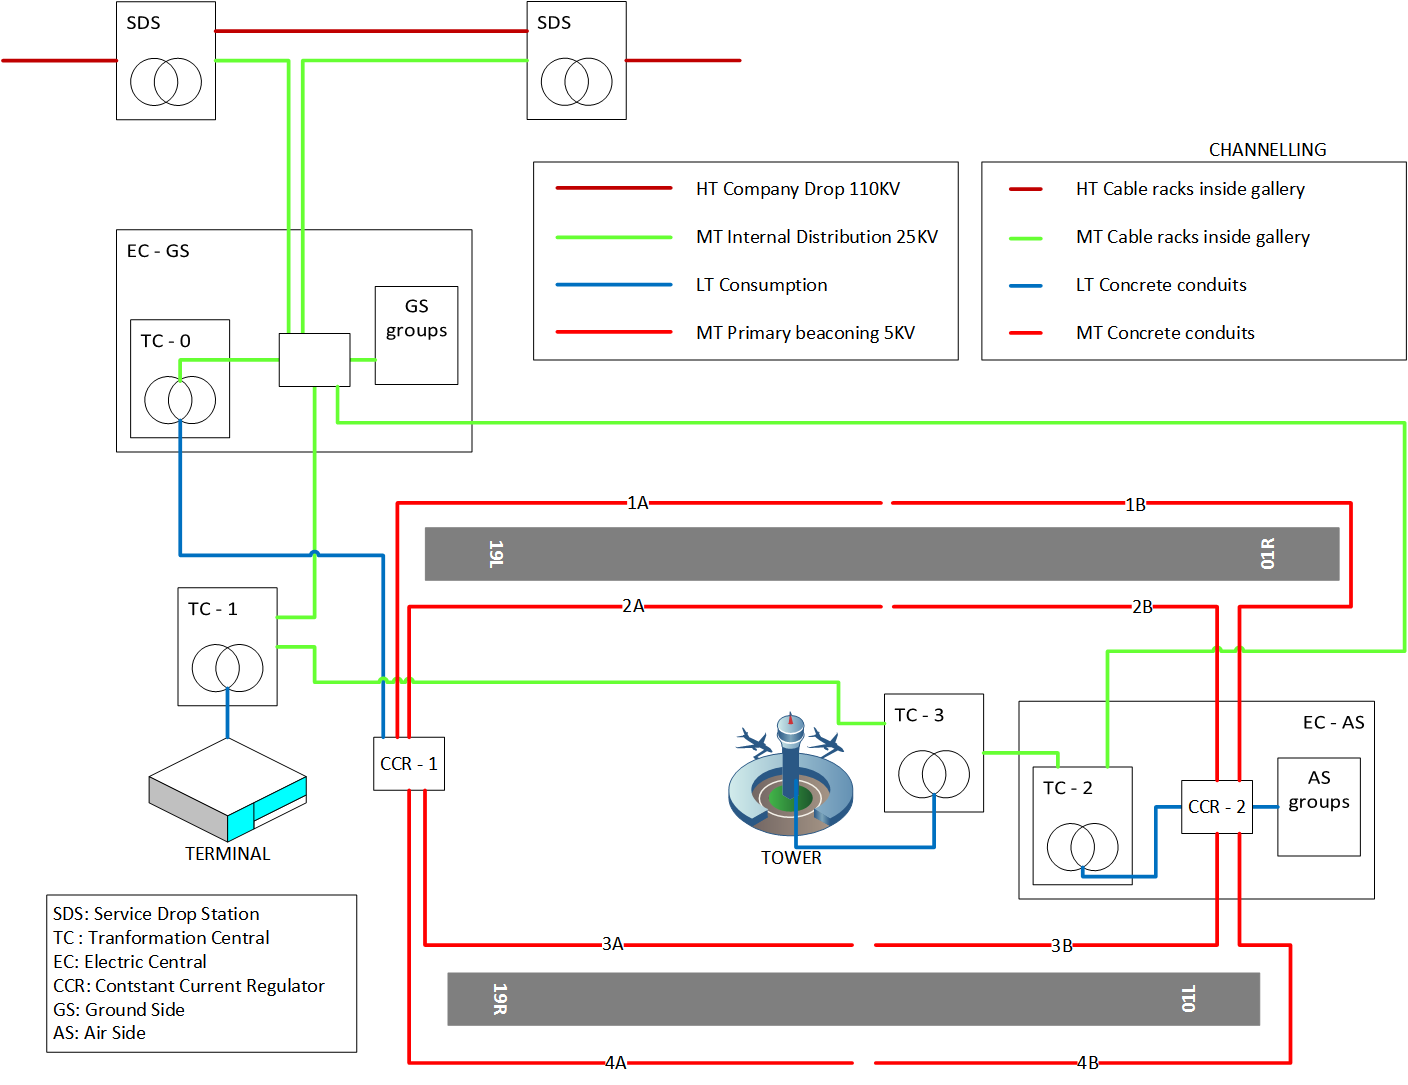
\includegraphics[clip, trim=0cm 0cm 0cm 0cm, width=0.5\textwidth]{./images/electric/esquema_electrico}
	\caption{General electric system scheme}
	\label{electricScheme}
\end{figure}

\section{PDF HORITZONTAL}
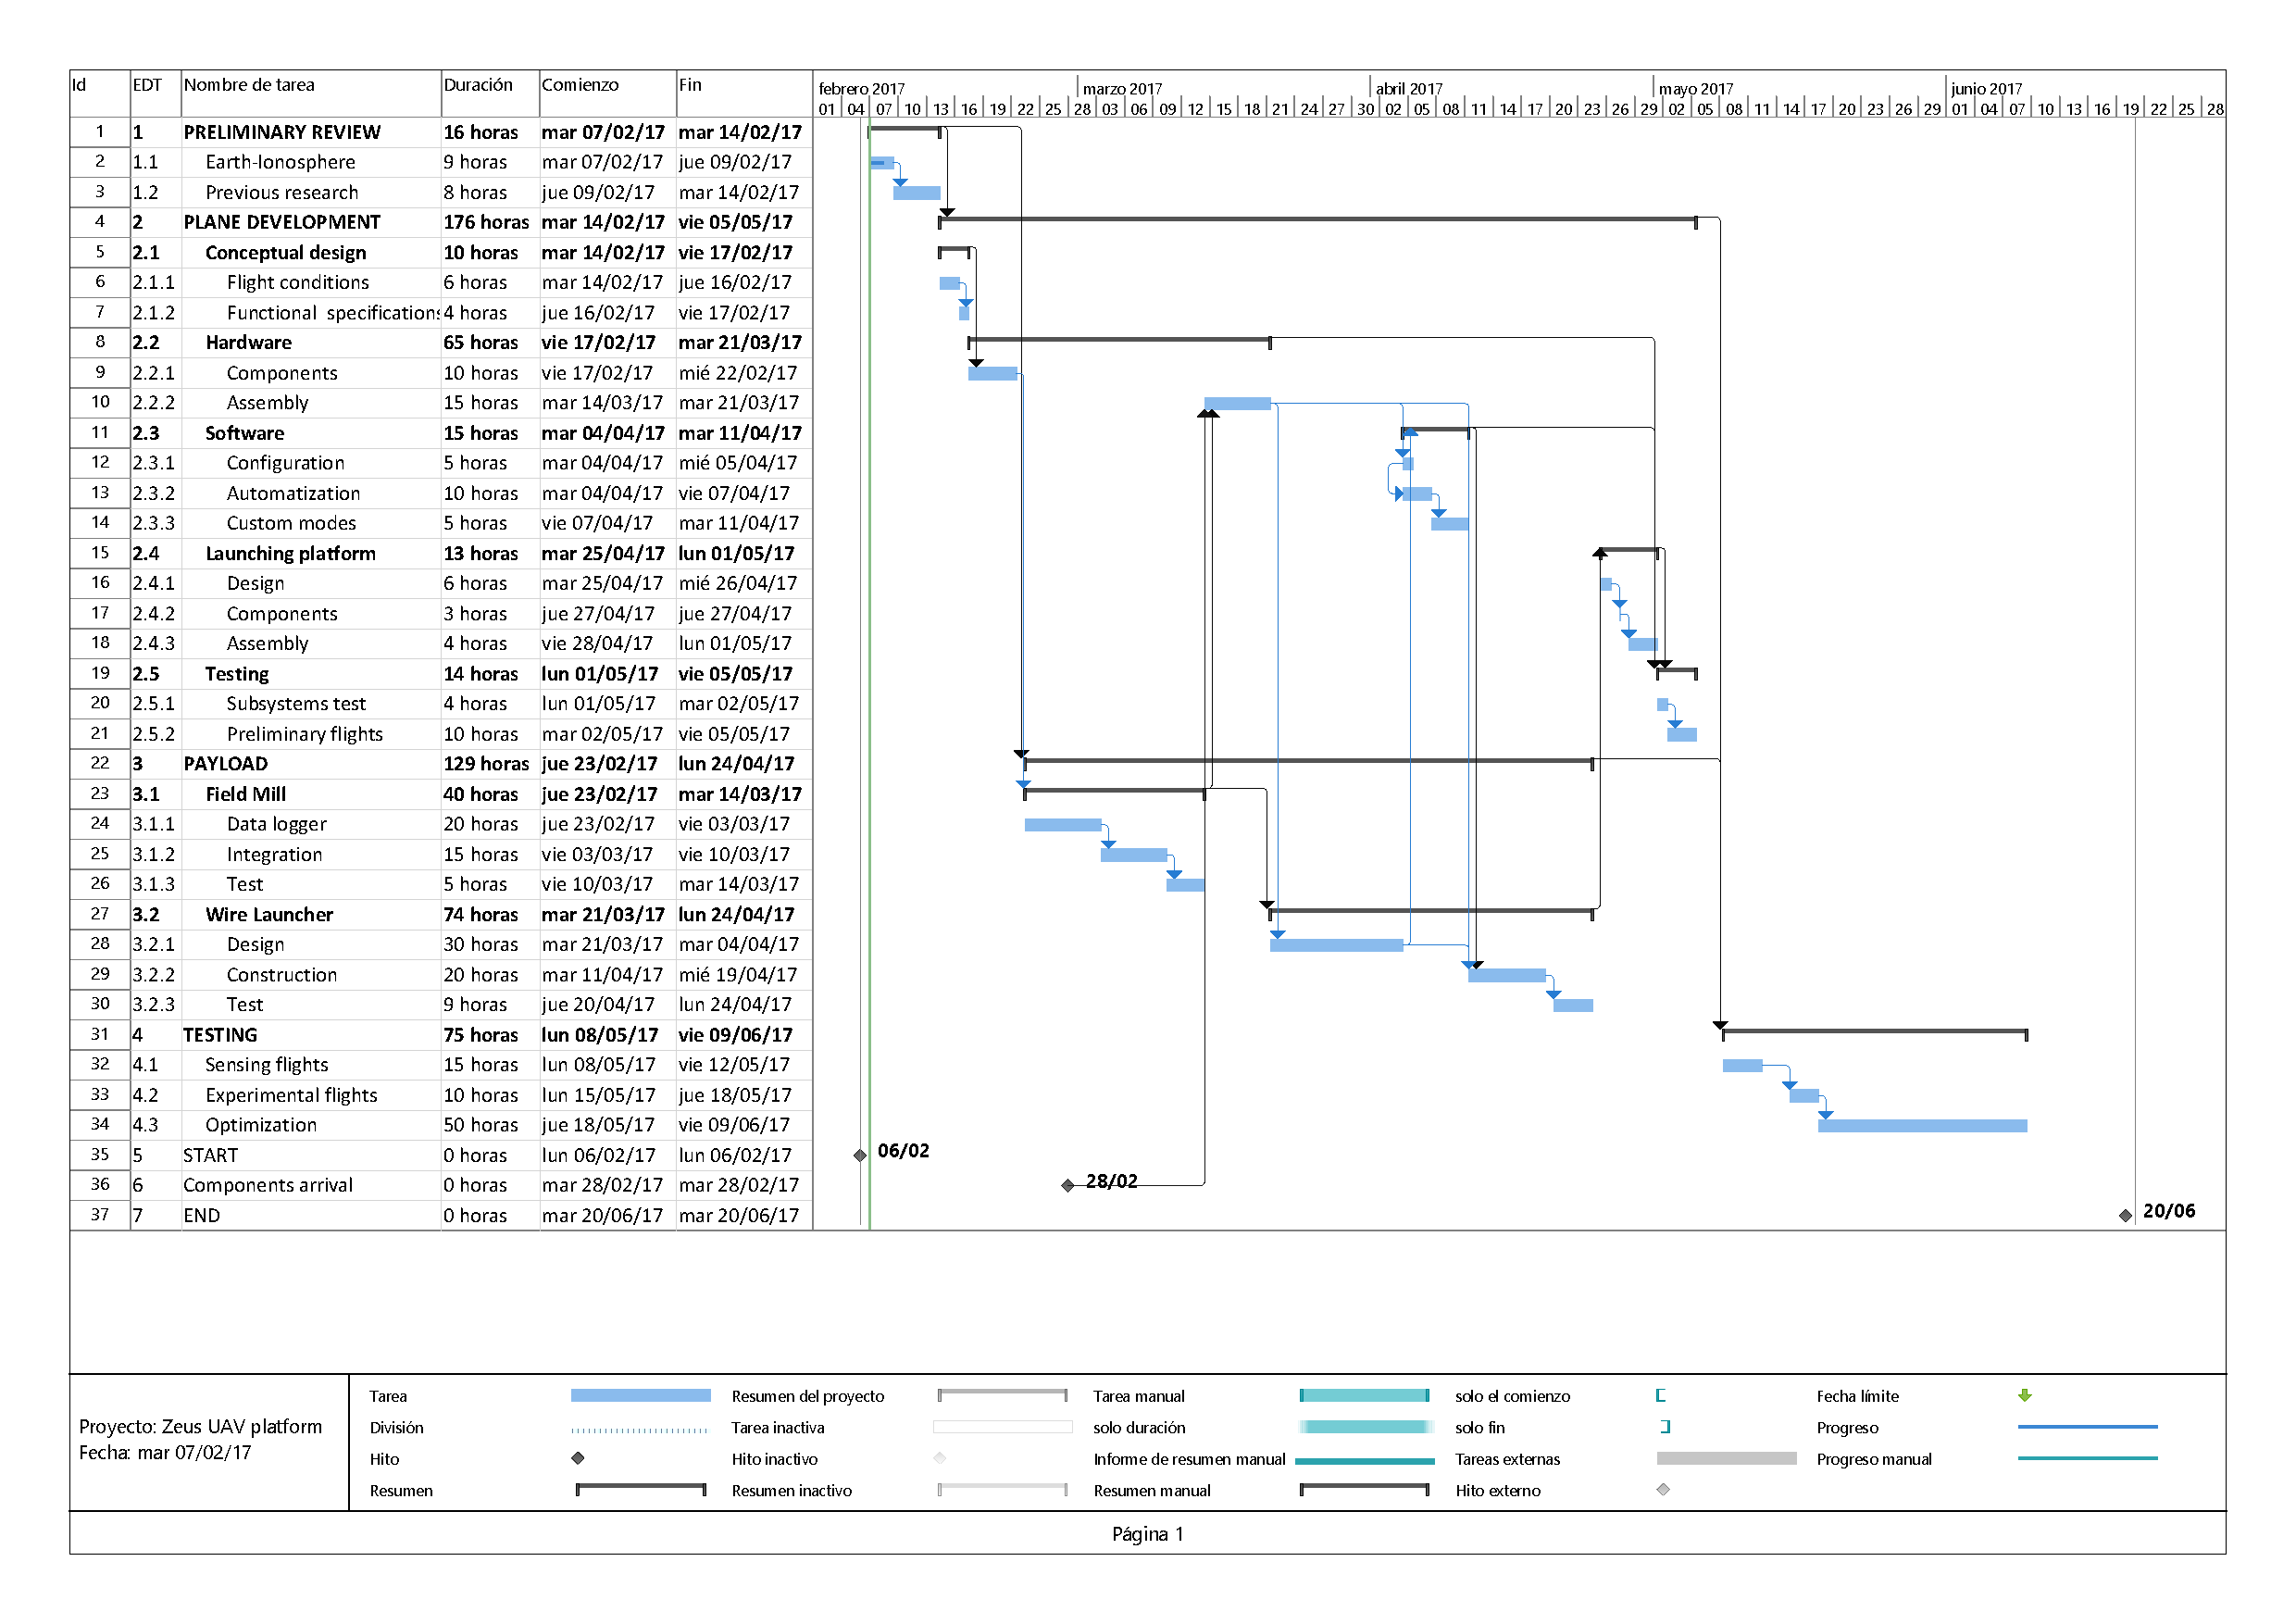
\includepdf[landscape=true]{./RAW/GANTT}


\chapter{Project Charter}
\section{Project Purpose and Justification}
\paragraph{} State the purpose of the project.  Tie the purpose to the organization's strategic goals and objectives if possible.  Tell the reader why this project is being started and what need is it fulfilling.  Identify if there are any specific mandates, policies or laws that are driving this change.

\subsection{Vision}
\paragraph{} The vision for this project shall be defined considering:

https://ec.europa.eu/research/participants/portal/desktop/en/opportunities/h2020/topics/lc-space-14-tec-2018-2019.html

\subsection{Objectives}

The key OBJECTIVES for this project are:

\begin{enumerate}

	\item Improve EO sensor's technologies in terms of reliability, size, resolution, efficiency and accuracy.

	\item Manufacture a technology demonstrator prototype.

	\item Simulate, test and validate the demonstrator prototype manufactured in relevant environment.

	\item Develop a data processing software with machine learning algorithms focused on urban sustainable development applications. 

	\item Develop a web based server for data sharing. 

	\item Provide a technology that helps urban sustainable development, improving the European society.
 
\end{enumerate}


	%\item Develop machine learning processing algorithms to enable automatic remote sensing based on urban sustainable development. 
\subsection{Scope}


The SCOPE for this project is:

{\bfseries Engineering} 
\begin{itemize}

	\item Research and analysis of the current space applications and requirements of the following optical and radar systems:

		\begin{itemize}

		\item LIDAR
		\item Radar
		\item Super-spectral
		\item Hyperspectral
		\item Limb sounders
		\item Gravimetry
		\item High quantum efficiency photodectectos
		\item High precisition optical beam scanning and pointing
		\item Advanced infrared technologies

		\end{itemize}

	\item Research of the contributions of current space technologies to urban development.

	\item Selection of the most promising systems to profit Earth Observation to air composition and terrain analysis.
	
	\item Development of sensor's preliminary design defining the minimum performance parameters in order to improve the existing technologies.

	\item ¿¿¿Interaction platform ???

	\item Development of a mock-up by following the preliminary design.

	\item Testing and validation of the prototype in a space simulated environment.

	\item Design closure and development of the product.

\end{itemize}

{\bfseries Business planning and exploitation of results}
\begin{itemize}
	\item Market analysis and of the potential suppliers and selection of these.
	\item Market analysis of the potential costumers.
	\item Elaboration of a business plan. 

\end{itemize}

\textbf{Quality} \textit{esto no acaba de parecer apropiado en el scope}
\begin{itemize}
	\item Every document goes through four stages to be approved:
	\begin{itemize}
		\item{-} Guidelines preparation
		\item{-} Document revision
		\item{-} Document rectification
		\item{-} Document approval
	\end{itemize}
	\item Elaboration of periodic reports in order to have continuous control over the development of the project.

\end{itemize}

\textbf{Communication and dissemination strategies} \textit{esto no acaba de parecer apropiado en el scope}

\begin{itemize}
	\item Implementation of a dissemination plan to announce the product combining online and offline dissemination.	
	 \item Development of 
	  a website. 
	  \item Use of social media marketing power. 
	  \item Conduct several conferences.
	  \item  Let to know the product improvements through technology demonstrators.
\end{itemize}





\section{Project Description}
As stated earlier, the main objective of the project is to enhance the performance of the EO systems so as to use the information derived from data to build a greener future. More specifically, the focus is on the improvement of both optical and radar systems and how can they contribute to the sustainable development of cities. 

To begin with, a research on the current technologies is carried out. This study makes it possible to determine which systems are more susceptible to further improvement. In order to demonstrate the advances in the aforementioned systems a prototype has to be manufactured and tested. 

Moreover, in the scope of this project, it has been included the development of a software that, once the data has been collected and received, treats the data in order to enable a more user-friendly data treatment on the final application and a web-based server for data sharing.

The project is grounded in initiatives such as the Copernicus programme. The Copernicus services aim at delivering nearly real-time data on a global level. This information allows us to better understand the planet we live in and secure a sustainable management of the environment. In fact, in context of the Copernicus, one of the previous H2020 calls has been involved in identifying possible potential evolutions of its space observation capabilities in order to build a climate resilient future. This call was focused on monitoring either the Polar Regions, agriculture or forests.

Among other things, Copernicus obtains data thanks to a set of dedicated satellites named Sentinel. Each of them has been developed for a specific need to provide accurate observation in each case. Nowadays, there is a total of six families of Sentinel. Hence, the idea is to take them a further step forward by equipping them with better remote sensing technologies. 

The different phases that constitute the project are summarized below:

\begin{enumerate}[label*=\arabic*.]
	\item STATE OF THE ART

This phase consists of a search on the state of the art technologies regarding payloads, modular systems and urban development applications of space technologies.
	
	\item PRODUCT DEVELOPMENT

The product development includes both a preliminary and a final design of the payloads, the modular system and the interaction platform. 
	
	\item SIMULATION, TESTING, VALIDATION, AND QUALITY

This phase includes the manufacturing of a technology demonstrator prototype, the validations of the payloads, the modular system, the interaction platform and the full system prototype. The quality of the product is also assured. 
	
\end{enumerate}


\newpage
\section{High-Level Requirements}

\subsection{Call for proposals requirements}
\begin{longtable}[H]{l c c}
	\toprule[2pt]
	\textbf{Item} &  \textbf{Description}                                                                                                                                               \\ \midrule
	C1 & \begin{tabular}[c]{@{}l@{}}\begin{minipage}[t]{\linewidth}
Contribute to the integration of space in society and economy. \vspace{0.3cm}
	\end{minipage} \end{tabular}                                                                                                                                            \\ \hline
	C2 & \begin{tabular}[c]{@{}l@{}}\begin{minipage}[t]{\linewidth}
			Improvement of state-of-the-art technologies in key areas. \vspace{0.3cm}
	\end{minipage} \end{tabular}                                                                                                                                            \\  \midrule
	C3 & \begin{tabular}[c]{@{}l@{}}\begin{minipage}[t]{\linewidth}
Enhancement of capabilities with respect to existing Earth observation missions. \vspace{0.3cm}
	\end{minipage} \end{tabular}                                                                                                                                          \\  \midrule
	C4 & \begin{tabular}[c]{@{}l@{}}\begin{minipage}[t]{\linewidth}
Complementarity with activities already funded by Member States and the European Space Agency \vspace{0.3cm}
	\end{minipage} \end{tabular}                                                                                                                                           \\  \midrule
	C5 & \begin{tabular}[c]{@{}l@{}}\begin{minipage}[t]{\linewidth}
Extend Europe's position in industrial competitiveness in technologies for Earth observation payloads and missions. \vspace{0.3cm}
	\end{minipage} \end{tabular}                                                                                                                                             \\  \midrule
	C6 & \begin{tabular}[c]{@{}l@{}}\begin{minipage}[t]{\linewidth}
			Promote industrial cooperation in research actions (including SMEs). \vspace{0.3cm}
	\end{minipage} \end{tabular}                                                                                                                                          \\  \midrule
	C7 & \begin{tabular}[c]{@{}l@{}}\begin{minipage}[t]{\linewidth}
			Promote networking between academia and industry, accelerating and broadening technology transfer. \vspace{0.3cm}
	\end{minipage} \end{tabular}                                                                                                                                             \\                                                                   	\bottomrule[2pt]
	\caption{Call of proposal requirements}
\end{longtable}

\subsection{Technical requirements}
\begin{longtable}[H]{l c c}
	\toprule[2pt]
	\textbf{Item} &  \textbf{Description}                                                                                                                                               \\ \midrule
	T1 & \begin{tabular}[c]{@{}l@{}}\begin{minipage}[t]{\linewidth}
			Ensure the endurance of the overall system. \vspace{0.3cm}
	\end{minipage} \end{tabular}                                                                                                                                            \\ \midrule
	T2 & \begin{tabular}[c]{@{}l@{}}\begin{minipage}[t]{\linewidth}
			Readiness for operational services. \vspace{0.3cm}
	\end{minipage} \end{tabular}                                                                                                                                            \\  \midrule
	T3 & \begin{tabular}[c]{@{}l@{}}\begin{minipage}[t]{\linewidth}
			Ability to detect greenhouse gases. \vspace{0.3cm}
	\end{minipage} \end{tabular}                                                                                                                                          \\  \midrule
	T4 & \begin{tabular}[c]{@{}l@{}}\begin{minipage}[t]{\linewidth}
			Ability to detect weather patterns for proper weather forecasting applications. \vspace{0.3cm}
	\end{minipage} \end{tabular}                                                                                                                                           \\  \midrule
	T5 & \begin{tabular}[c]{@{}l@{}}\begin{minipage}[t]{\linewidth}
			Ability to perform a high precision terrain mapping for urban applications. \vspace{0.3cm}
	\end{minipage} \end{tabular}                                                                                                                                             \\  \midrule
	T6 & \begin{tabular}[c]{@{}l@{}}\begin{minipage}[t]{\linewidth}
			The system must have a program for automatic updates and self-revision of possible issues. \vspace{0.3cm}
	\end{minipage} \end{tabular}                                                                                                                                          \\  \midrule
	T7 & \begin{tabular}[c]{@{}l@{}}\begin{minipage}[t]{\linewidth}
			Availability of real-time information with a maximum delay of 1 second. \vspace{0.3cm}
	\end{minipage} \end{tabular}
	\\ \midrule
	T8 & \begin{tabular}[c]{@{}l@{}}\begin{minipage}[t]{\linewidth}
			15\% increase of the reliability and precision of results compared to current technologies. \vspace{0.3cm}
	\end{minipage} \end{tabular}                                                                                                                                             \\                                                                   	\bottomrule[2pt]
	\caption{Technical requirements}
\end{longtable}
\section{Acceptance Criteria}

The acceptance criteria are important to define the performance requirements and the essential conditions that the deliverables of the project must attain. It is a quality parameter and the fact that they are fulfilled indicates that the client's needs have been reached.

\begin{center}
	\begin{tabular}{|p{2cm}|p{10cm}|}
		\hline 
		Research and innovation & The project must be ambitious and use all available resources to obtain the best result. In this way, it must include the most appropriate technology that there is so far and, if it is in the development phase, add a section of research. 
		\\ 
		\hline 
		Quality & The content of the project documentation must be clear, complete and understandable. Furthermore, it must be well structured, dividing the information into approach, development and conclusions.
		All the documentation included in the project must first pass through an inspection of the quality department. 
		\\ 
		\hline 
		Test and validations & The evaluation and validation tests must be carried out periodically and be registered in the project documentation, in such a way that there is a record of the different versions of the application throughout the development.
		The information of these tests must be presented clearly and refer to the regulations concerned, in addition to be verifiable.
		The results of these tests should be used to analyze the service level of the application and improve on later versions.
		\\ 
		\hline 
		Technical documents & The application must have a user manual both internally and externally and attach the necessary information for its development.
		The performance of the final product must be reflected in a data sheet, it must also include in the documentation the datasheet of the different components that are part of the application.
		\\ 
		\hline
		Viability & The project must be viable economically and technically, so that its realization is possible.
		The different parts of the project must be submitted at the individual level to a study that checks if it is possible to do them and, if not, search for an alternative.
		The budget of the project must comply with the financial requirements of the European Union, for which must be make a balance to ensure that the allowed limit is not exceeded.
		\\ 
		\hline 
		Performance & The systems used in the project must be able to guarantee the right functioning of the application. An important aspect of the project is its performance, in this way, as it progresses, it aims to increase the efficiency and quantify this increase in the different phases. 
		\\ 
		\hline 
		Collaboration & It is interesting to obtain a better result to collaborate with legal entities from different countries, as universities and research groups. Moreover, different collaborations with SMEs should be tried, in addition to they can benefit in turn and grow in the market. 
		\\ 
		\hline
		Transparency & In case information about the project is required by the part of official organizations of the European Union or by the different stakeholders that participate in it, the information must be shared with transparency. 
		\\ 
		\hline
		Legal requirements and ethical code & The applications and products of this project must have, if required, the certification and approval of the different legislative and ethical frameworks. \\ 
		\hline
		
	\end{tabular} 
\end{center}
\section{High-Level Risks}

Risks allow us to measure the probability of not accomplishing a defined goal and its consequences for the project. Their identification is crucial in order to know in advance the factors that could make the project go wrong.

The determination of the risks is an iterative process because, when the different activities progress through the specified time, new risks or uncertainties can appear. The main structures and departments of the team have to participate in this task in order to spot as many risks as possible. Even stakeholders have to provide additional information and points of view.

The factors that are used in the identification process are: enterprise environmental factors, organizational process assets, the project scope statement and the project management plan.

After analysing these points, risks have been classified in two groups: External risks, which are the ones that our team cannot control, so they are inevitable, and Internal risks, which can be detected in advance and be addressed properly by our own members.

The main identified risks are shown below.

\textbf{External risks}

\begin{itemize}
	
	\item \textbf{Competitors appearance:} The emergence of other companies that could offer the same product. This could modify the benefits of our company.
	
	\item \textbf{Delays in external deliverables:} If the products that the company orders do not arrive at the predicted time all the processes can experience a delay, incrementing costs.
	
	\item \textbf{Economical market issues:} During the period of time that the project is executed, there could be large-scale economic crisis.
	
	\item \textbf{Exit of a member of the corporation:} For different reasons, a member that had committed to the project could leave it before than expected.
	
	\item \textbf{Components and raw materials quality:} The ordered equipment or materials could not be in good condition, delaying processes and increasing costs.
	
\end{itemize}

\textbf{Internal risks}

\begin{itemize}
	
	\item \textbf{Delays in deliverables:} The deliverables could not be completed at the time of their corresponding deadlines, leading to an increase of costs and a delay of all the schedule of the project.
	
	\item \textbf{Cost forecasts are inaccurate:} The financial predictions could be wrong or different issues may occur increasing the total cost of the project.
	
	\item \textbf{Lack of communication:} The absence of a proper communication method or channel might affect the quality of the product, the fulfilment of the deadlines or a good coordination between members and departments.
	
	\item \textbf{Lack of technology improvement:} The main goal of the project is to innovate but it could happen that the company did not find the way to improve enough the different technologies.
	
	\item \textbf{Lack of information:} Discovering new technologies implies working with leading-edge science. It could occur that the team does not have access to the last improvements or patents.
	
	\item \textbf{Low team motivation:} The team could lose motivation, which would lead the project to take more time and costs to be completed.
	
	\item \textbf{Unsuccessful quality control:} The quality of some component, product or deliverable may not be as it is expected and established in the acceptance criteria.
	
	\item \textbf{Lack of responsibilities:} The responsibilities taken by the members of the team or the stakeholders could not be accomplished as expected.
	
	\item \textbf{Conflicts between members:} There could be a disagreement over the project issues between executive members.
	
	\item \textbf{Infeasible design:} The design could turn out to be excessively costly or not possible to be built.
	
	\item \textbf{Technology components have security vulnerabilities:} Security vulnerabilities are unwanted in high-tech projects if some government is interested in using the technology.
	
	\item \textbf{Organization issues:} The project could be not well organized in terms of timing, activities, etc. and the schedule may be always changing.
	
	\item \textbf{Stakeholders desertion:} The abandonment of a stakeholder could occur for several reasons, leaving the project without its contribution.
	
	\item \textbf{Stakeholders conflict:} Different executives of the stakeholders could have a disagreement over the project at an executive level.
	
	
\end{itemize}

When managing risks, both the probability and their consequences have to be considered. During the project, each event will be classified into different types of risks. In a general level, they can be classified into low, moderate and high risks. The following figure represents the classification depending on the probability and the magnitude of impact.

\begin{figure}[H]
	\centering
	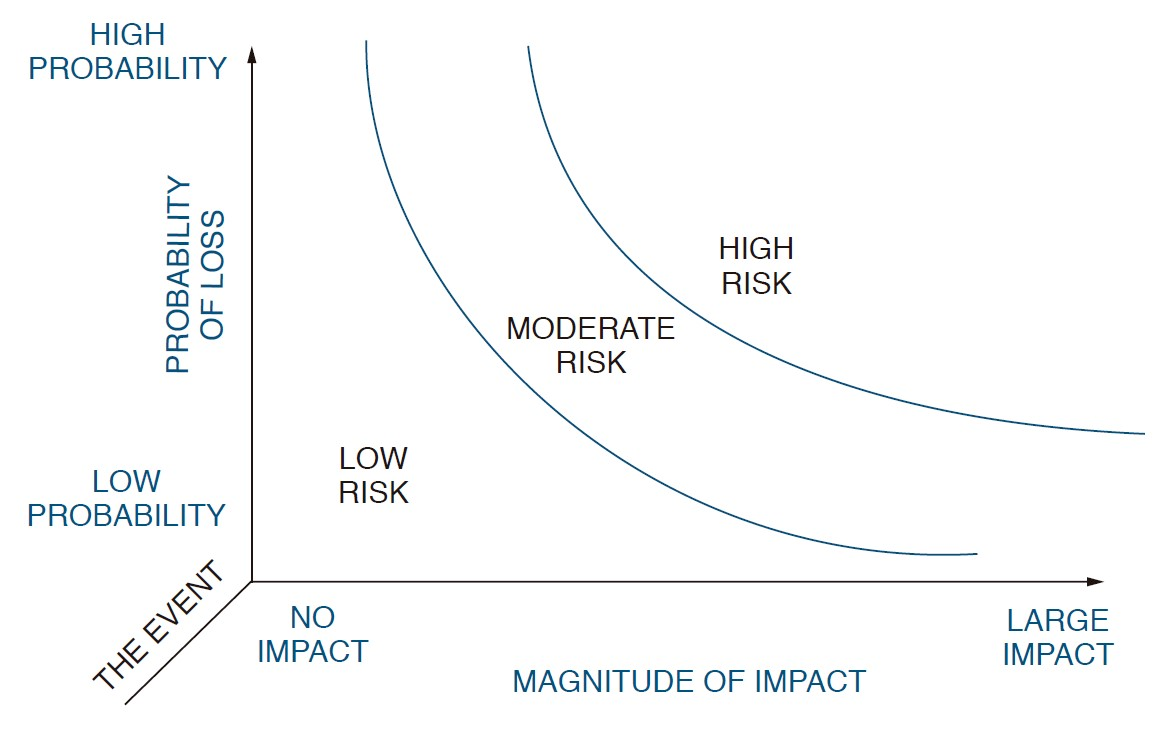
\includegraphics[width=0.65\linewidth]{./images/risks1}
	\caption{Overall risk is a function of its components \cite{Kerzner2009}.}
	\label{fig:risks1}
\end{figure}

During the following stages of the project, each risk will be assessed with the Probability and Impact Matrix. It is a tool which allows the team to rate risks on their probability and impact in the project. This gives a quick and clear view of which risk is more important to control.

\begin{figure}[H]
	\centering
	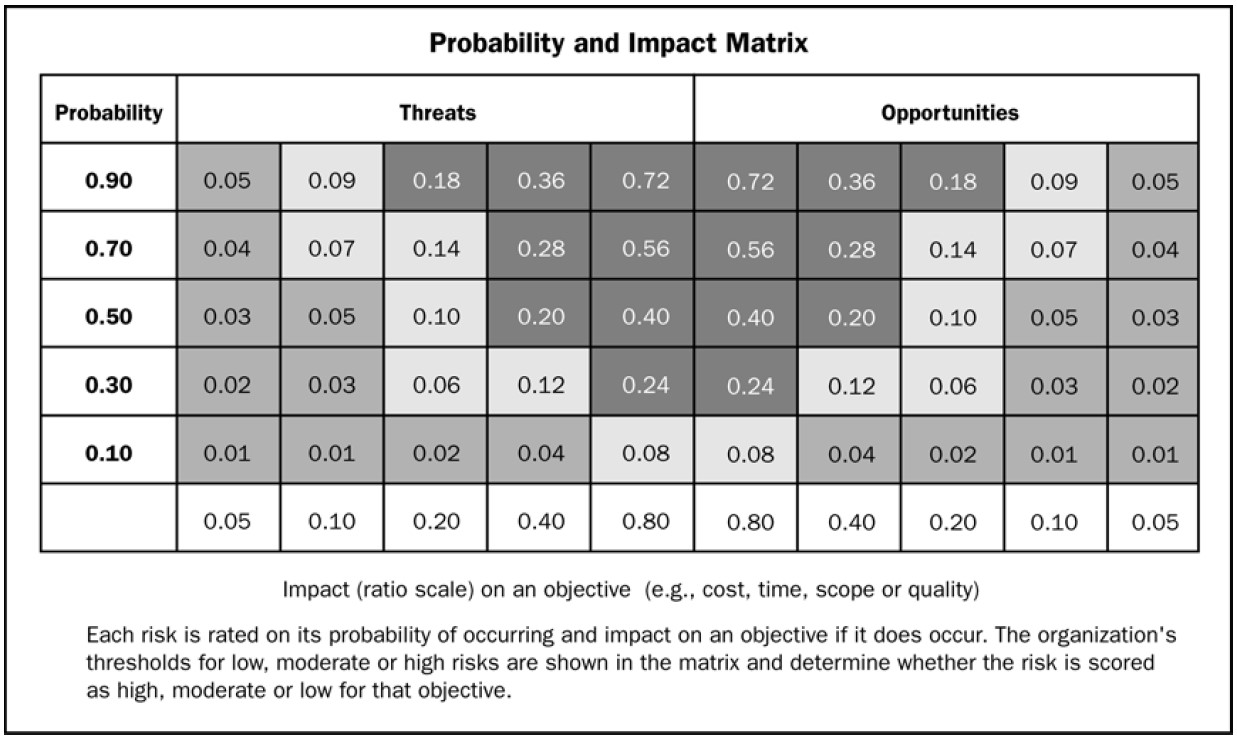
\includegraphics[width=\linewidth]{./images/risks2}
	\caption{Probability and Impact Matrix \cite{ProjectManagementInstitute2004}.}
	\label{fig:risks2}
\end{figure}


\section{Project deliverables}

\begin{longtable}[H]{l p{6cm} c}
	\toprule[2pt]
	\textbf{Deliverable Name} &  \textbf{Description}  & \textbf{Estimated due date}                                                                                                                                                        \\ \midrule
	Project management plan & \begin{tabular}[c]{@{}l@{}}\begin{minipage}[t]{\linewidth}
		Document with detailed explanation of the project management strategies, including the Project Charter, stakeholder register, risk, quality and financial plans. \vspace{0.3cm}
	\end{minipage} \end{tabular}   & $t_0 +1$ month                                                                                                                                           \\ \hline
	Business plan & \begin{tabular}[c]{@{}l@{}}\begin{minipage}[t]{\linewidth}
			Document detailing the market approach, including the selected suppliers, the identified costumers and the exploitation strategy. \vspace{0.3cm}
	\end{minipage} \end{tabular}   & $t_0 +1$ month                                                                                                                                           \\  \midrule
	Communication plan & \begin{tabular}[c]{@{}l@{}}\begin{minipage}[t]{\linewidth}
			Document containing all the planned dissemination strategies, such as the online communication (including website development and social media management), the offline communication (participation in meetings and conferences) and the dissemination materials (technology demonstrators). \vspace{0.3cm}
	\end{minipage} \end{tabular}   & $t_0 +1$ month                                                                                                                                           \\ \midrule
	State of the art report & \begin{tabular}[c]{@{}l@{}}\begin{minipage}[t]{\linewidth}
			Report detailing the current state of the art and the study of requirements for each system of the project. \vspace{0.3cm}
	\end{minipage} \end{tabular}   & $t_0 +4$ month                                                                                                                                           \\  \midrule
	Preliminary design report & \begin{tabular}[c]{@{}l@{}}\begin{minipage}[t]{\linewidth}
			Report determining the preliminary performance parameters of each sensor, as well as the technology necessary for the overall system. \vspace{0.3cm}
	\end{minipage} \end{tabular}   & $t_0 +16$ month                                                                                                                                           \\  \midrule
	Mid-term project report & \begin{tabular}[c]{@{}l@{}}\begin{minipage}[t]{\linewidth}
			Document used to check the current state of the project, in order to inform all the participants, including the stakeholders, of the progress. \vspace{0.3cm}
	\end{minipage} \end{tabular}   & $t_0 +17$ month                                                                                                                                           \\  \midrule
	Final design report & \begin{tabular}[c]{@{}l@{}}\begin{minipage}[t]{\linewidth}
			Report detailing the final design and technical specifications of each sensor developed, the software of the system and the interaction platform. \vspace{0.3cm}
	\end{minipage} \end{tabular}   & $t_0 +29$ month                                                                                                                                           \\  \midrule
	Validation report & \begin{tabular}[c]{@{}l@{}}\begin{minipage}[t]{\linewidth}
			Report gathering the results obtained from the fabrication and testing of all the payload sensors, the modular system and the interaction platform, as well as the full system testing. \vspace{0.3cm}
	\end{minipage} \end{tabular}   & $t_0 +41$ month                                                                                                                                           \\  \hline
	Final report & \begin{tabular}[c]{@{}l@{}}\begin{minipage}[t]{\linewidth}
			Final document delivered, that includes all the development done through the execution of the project. \vspace{0.3cm}
	\end{minipage} \end{tabular}   & $t_0 + 44$ month                                                                                                                                           
	
		\\ \bottomrule[2pt]
	\caption{Project Deliverables}
\end{longtable}



\section{Project milestones}
\begin{longtable}[H]{p{5cm} p{8cm} c}
	\toprule[2pt]
	\textbf{Milestones Name} &  \textbf{Description}  & \textbf{Estimated due date}                                                                                                                                                        \\ \midrule
	Kick-Off Meeting & \begin{tabular}[c]{@{}l@{}}\begin{minipage}[t]{\linewidth}
			First meeting of the project, formation of the development team and first contact with the stakeholders. \vspace{0.3cm}
	\end{minipage} \end{tabular}   & $t_0$ month                                                                                                                                           \\ \hline
	Project management plan & \begin{tabular}[c]{@{}l@{}}\begin{minipage}[t]{\linewidth}
			Specification of the objectives and scope of the project, the organization of the team and the distribution of tasks, a stakeholders register and a financial, quality and risk plans. \vspace{0.3cm}
	\end{minipage} \end{tabular}   & $t_0 +1$ month                                                                                                                                           \\ \hline
	Business plan & \begin{tabular}[c]{@{}l@{}}\begin{minipage}[t]{\linewidth}
			Obtaining a potential suppliers list, and negotiating procurement conditions with them, as well as identifying and communicating with potential customers. \vspace{0.3cm}
	\end{minipage} \end{tabular}   & $t_0 +1$ month                                                                                                                                           \\  \midrule
	Communication plan & \begin{tabular}[c]{@{}l@{}}\begin{minipage}[t]{\linewidth}
			Development of a website and a social media strategy, as well as looking into participation in meetings and conferences. \vspace{0.3cm}
	\end{minipage} \end{tabular}   & $t_0 +1$ month                                                                                                                                           \\
	Research report & \begin{tabular}[c]{@{}l@{}}\begin{minipage}[t]{\linewidth}
			Definition of requirements for the system based on the current state of the art space applications of the payload sensors. \vspace{0.3cm}
	\end{minipage} \end{tabular}   & $t_0 +4$ month                                                                                                                                           \\  \midrule  
	Payload preliminary design & \begin{tabular}[c]{@{}l@{}}\begin{minipage}[t]{\linewidth}
			First phase of the design, an optimization of each sensor is done in order to define the preliminary minimum performance parameters. \vspace{0.3cm}
	\end{minipage} \end{tabular}   & $t_0 +10$ month                                                                                                                                           \\ \midrule
	Modular system preliminary design & \begin{tabular}[c]{@{}l@{}}\begin{minipage}[t]{\linewidth}
			Development of the initial parameters of the modular system, as well as the software that will be in charge of the fusion of the sensors’ data. \vspace{0.3cm}
	\end{minipage} \end{tabular}   & $t_0 +13$ month                                                                                                                                           \\ \midrule                                                                                                                                  
	Interaction platform preliminary design & \begin{tabular}[c]{@{}l@{}}\begin{minipage}[t]{\linewidth}
			Preliminary implementation of the functionalities of the interaction platform, such as the machine learning algorithms.  \vspace{0.3cm}
	\end{minipage} \end{tabular}   & $t_0 +16$ month                                                                                                                                           \\ \midrule
	Mid-term project report & \begin{tabular}[c]{@{}l@{}}\begin{minipage}[t]{\linewidth}
			Mid-term report to evaluate and validate by all the stakeholders the status of the project.  \vspace{0.3cm}
	\end{minipage} \end{tabular}   & $t_0 +17$ month                                                                                                                                           \\ \midrule
	Payload final design & \begin{tabular}[c]{@{}l@{}}\begin{minipage}[t]{\linewidth}
			Final design of the entire payload (sensors), including the specifications and estimated performance in operation of each sensor.  \vspace{0.3cm}
	\end{minipage} \end{tabular}   & $t_0 + 23$ month                                                                                                                                           \\ \midrule
	Modular system final design & \begin{tabular}[c]{@{}l@{}}\begin{minipage}[t]{\linewidth}
			Final design of the modular system and the software that will process and register the information received by the payload. \vspace{0.3cm}
	\end{minipage} \end{tabular}   & $t_0 + 26$ month                                                                                                                                           \\ \midrule
	Interaction platform final design & \begin{tabular}[c]{@{}l@{}}\begin{minipage}[t]{\linewidth}
		Final design of the interaction platform according to the guidelines stablished on the preliminary design. \vspace{0.3cm}
	\end{minipage} \end{tabular}   & $t_0 + 29$ month                                                                                                                                           \\ \midrule
	Prototype manufacturing & \begin{tabular}[c]{@{}l@{}}\begin{minipage}[t]{\linewidth}
		Manufacturing of the prototype according to the final designs, in order to test its function in the next steps.  \vspace{0.3cm}
	\end{minipage} \end{tabular}   & $t_0 + 34$ month                                                                                                                                           \\ \midrule
	Individual systems testing & \begin{tabular}[c]{@{}l@{}}\begin{minipage}[t]{\linewidth}
		Performance analysis of each module (payload, modular system and interaction platform) of the overall system under operational conditions.\vspace{0.3cm}
	\end{minipage} \end{tabular}   & $t_0 + 37$ month
	
	\\ \bottomrule[2pt]
	\caption{Project Milestones}
\end{longtable}

\section{Project Objectives}
\begin{center}
	\begin{longtable}{>{\raggedright\arraybackslash}p{5cm} >{\raggedright\arraybackslash}p{5cm} >{\raggedleft\arraybackslash}p{2.5cm}}
		\toprule[2pt]
		\textbf{Project Objectives} & \textbf{Success Criteria} & \textbf{Approval Responsible} \\
		\midrule \endhead
		\textbf{Scope} &  &  \\
		\hline
		Introduction and demonstration of new technologies, systems and sub-systems for EO (Earth Observation). & The systems must prove their proper functioning in a relevant environment and be able to provide the user the required data. & Project Manager \\
		\hline
		\textbf{Time} &  &   \\
		\hline
		44 months & After the analysis of project deliverables and project milestones, a period of 44 months seems acceptable. Nevertheless, possible delays may appear during the project development. Hence, proper time-management is necessary to complete the project within the aimed duration. & Project Manager  \\
		\hline
		\textbf{Cost} &  &   \\
		\hline
		4 million \euro & The estimated cost of the project is 4M  and it is detailed in the next section. Every expense of the project must be controlled and limited to avoid exceeding the budget. & Financial Manager  \\	
		\hline
		\textbf{Quality} &  &   \\
		\hline
		Organised, planned and detailed development with continuous improvement & 
 Elaboration of periodic reports in order to have continuous control over the development of the project. \newline
 Documentation must be complete, understable and structured.
 
 		& Quality Manager  \\	
		\bottomrule[2pt]
		\caption{Project Objectives}
	\end{longtable}
\end{center}

\section{Estimated Budget}

The financial resources required for the completion of the project are expected to be covered by the contribution of the EU Commission.\\

The estimated budget is 4,000,00.00 \EUR, which is calculated taking into account the requirement for each stakeholder in order to complete the parts assigned to it. The next table shows the resources required for each stakeholder.


% Table of Breakdown of the project budget
% \begin{table}[H]
% \centering
% \caption{Breakdown of the project budget (units in euros).}
% \label{my-label}
% \scalebox{0.6}{
% \begin{tabular}{p{5cm}p{2cm}p{2cm}p{2cm}p{2cm}p{2cm}p{2cm}p{2cm}p{2cm}}
% \toprule[2pt]
% \textbf{Participant short name}                                                                      & \textbf{(A) Direct Personnel costs} & \textbf{(B) Other Direct Costs} & \textbf{(C) Direct costs of sub-  contracting} & \textbf{(F) Indirect costs} & \textbf{(H) Total estimated eligible costs} & \textbf{(I) Reimbourse- ment Rate (\%)} & \textbf{(J) Max. EU Contribution} & \textbf{(K) Requested EU Contribution} \\ \hline 
% \textbf{HIRO}  & 140,000   & 15,000    & 6,250   & 38,750   & 200,000  & 100 \%  & 200,000  & 200,000  \\
% \textbf{Airbus Defence and Space GmbH}       & 200,000                                                                                               & 120,000                                                                                         &0                                                                                             & 80,000                                                                                     & 400,000                                                                                                    & 100\%                                                                                                & 400,000                                                                                             & 400,000                                                                                               \\
% \textbf{BHO Legal Rechtsanwälte Partnership} & 75,000                                                                                                & 5,000                                                                                           &0                                                                                                                & 20,000                                                                                     & 100,000                                                                                                    & 100\%                                                                                                & 100,000                                                                                             & 100,000                                                                                               \\
% \textbf{Deimos Space S.L.U.}                 & 495,000                                                                                               & 385,000                                                                                         &0                                                                                                                & 220,000                                                                                    & 1,100,000                                                                                                  & 100\%                                                                                                & 1,100,000                                                                                           & 1,100,000                                                                                             \\
% \textbf{ICUBE-SERTIT}                                                                    & 250,000                                                                                               & 150,000                                                                                         &0                                                                                                                & 100,000                                                                                    & 500,000                                                                                                    & 100\%                                                                                                & 500,000                                                                                             & 500,000                                                                                               \\
% \textbf{ReSAC}                                                                           & 45,000                                                                                                & 35,000                                                                                          &0                                                                                                                & 20,000                                                                                     & 100,000                                                                                                    & 100\%                                                                                                & 100,000                                                                                             & 100,000                                                                                               \\
% \textbf{Thales Alenia Space SAS}             & 840,000                                                                                               & 280,000                                                                                         &0                                                                                                                & 280,000                                                                                    & 1,400,000                                                                                                  & 100\%                                                                                                & 1,400,000                                                                                           & 1,400,000                                                                                             \\
% \textbf{VITO nv.}                                                                        & 90,000                                                                                                & 70,000                                                                                          &0                                                                                                                & 40,000                                                                                     & 200,000                                                                                                    & 100\%                                                                                                & 200,000                                                                                             & 200,000                                                                                               \\\hline
% \textbf{TOTAL}                                                                           & \textbf{2,135,000}                                                                                    & \textbf{1,060,000}                                                                              & \textbf{6,250}                                                                                                 & \textbf{798,750}                                                                           & \textbf{4,000,000}                                                                                         & \textbf{}                                                                                            & \textbf{4,000,000}                                                                                  & \textbf{4,000,000}                                                                                   
% \\ \bottomrule[2pt]
% \end{tabular}}
% \end{table}


\begin{figure}[H]
\centering
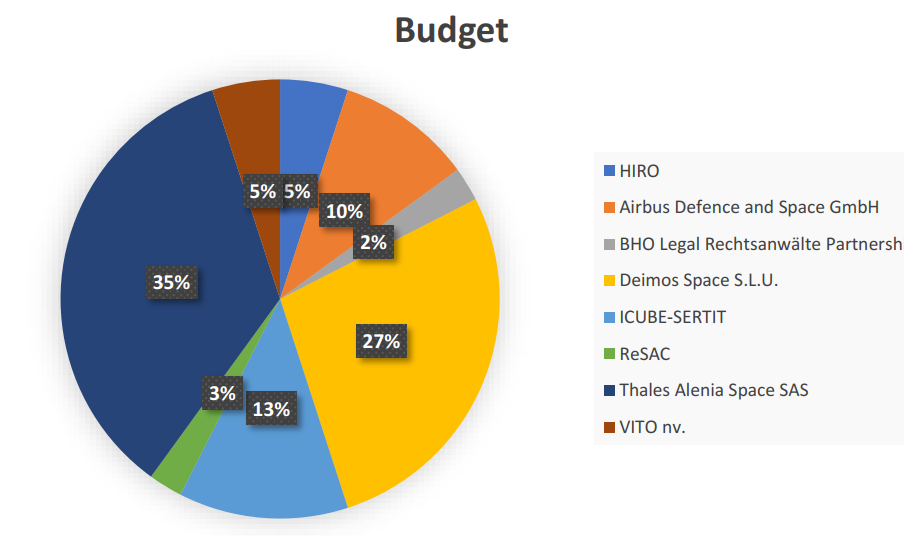
\includegraphics[scale=0.5]{./images/budget/budgetPie}
\caption{Percentage breakdown of the project expenses.}
\label{rules}
\end{figure}

The breakdown of the expenses for each organization is shown in more detail in the following tables. Six generic departments are set up for each organization involved: management, engineering, marketing, partnership and networks, contingencies and manufacturing. However, not all the organizations are constituted by all of these departments as each organization has a unique purpose which can make the contributions to departments such as manufacturing inexistent.\\

% Results table

% New packages
% \usepackage{rotating}
% \usepackage{pdflscape} % for 'landscape' environment

% % Results table

% New packages
% \usepackage{rotating}
% \usepackage{pdflscape} % for 'landscape' environment

% \input{./tab_results}

 %\endfirsthead

\newpage
\begin{landscape}\tiny
     \begin{table}[H]
    \centering
    \caption{Breakdown of the project budget (units in euros).}
    \label{my-label}
    \scalebox{0.6}{
    \begin{tabular}{p{5cm}p{5cm}p{5cm}p{5cm}p{5cm}p{5cm}p{5cm}p{5cm}p{5cm}}
    \toprule[2pt]
    \textbf{Participant short name}                                                                      & \textbf{(A) Direct Personnel costs} & \textbf{(B) Other Direct Costs} & \textbf{(C) Direct costs of sub-contracting} & \textbf{(F) Indirect costs} & \textbf{(H) Total estimated eligible costs} & \textbf{(I) Reimboursement Rate (\%)} & \textbf{(J) Max. EU Contribution} & \textbf{(K) Requested EU Contribution} \\ \hline 
    \textbf{HIRO}  & 140,000   & 15,000    & 6,250   & 38,750   & 200,000  & 100 \%  & 200,000  & 200,000  \\
    \textbf{Airbus Defence and Space GmbH}       & 200,000                                                                                               & 120,000                                                                                         &0                                                                                             & 80,000                                                                                     & 400,000                                                                                                    & 100\%                                                                                                & 400,000                                                                                             & 400,000                                                                                               \\
    \textbf{BHO Legal Rechtsanwälte Partnership} & 75,000                                                                                                & 5,000                                                                                           &0                                                                                                                & 20,000                                                                                     & 100,000                                                                                                    & 100\%                                                                                                & 100,000                                                                                             & 100,000                                                                                               \\
    \textbf{Deimos Space S.L.U.}                 & 495,000                                                                                               & 385,000                                                                                         &0                                                                                                                & 220,000                                                                                    & 1,100,000                                                                                                  & 100\%                                                                                                & 1,100,000                                                                                           & 1,100,000                                                                                             \\
    \textbf{ICUBE-SERTIT}                                                                    & 250,000                                                                                               & 150,000                                                                                         &0                                                                                                                & 100,000                                                                                    & 500,000                                                                                                    & 100\%                                                                                                & 500,000                                                                                             & 500,000                                                                                               \\
    \textbf{ReSAC}                                                                           & 45,000                                                                                                & 35,000                                                                                          &0                                                                                                                & 20,000                                                                                     & 100,000                                                                                                    & 100\%                                                                                                & 100,000                                                                                             & 100,000                                                                                               \\
    \textbf{Thales Alenia Space SAS}             & 840,000                                                                                               & 280,000                                                                                         &0                                                                                                                & 280,000                                                                                    & 1,400,000                                                                                                  & 100\%                                                                                                & 1,400,000                                                                                           & 1,400,000                                                                                             \\
    \textbf{VITO nv.}                                                                        & 90,000                                                                                                & 70,000                                                                                          &0                                                                                                                & 40,000                                                                                     & 200,000                                                                                                    & 100\%                                                                                                & 200,000                                                                                             & 200,000                                                                                               \\\hline
    \textbf{TOTAL}                                                                           & \textbf{2,135,000}                                                                                    & \textbf{1,060,000}                                                                              & \textbf{6,250}                                                                                                 & \textbf{798,750}                                                                           & \textbf{4,000,000}                                                                                         & \textbf{}                                                                                            & \textbf{4,000,000}                                                                                  & \textbf{4,000,000}                                                                                   
    \\ \bottomrule[2pt]
    \end{tabular}}
    \end{table}

    \begin{table}[H]
    \centering
    \caption{Cost details in euros for HIRO.}
    \label{my-label}
    \scalebox{0.6}{
    \begin{tabular}{p{5cm}p{2cm}p{2cm}p{2.5cm}p{2cm}p{2cm}p{2cm}p{2cm}p{2cm}}
    \toprule[2pt] 
    \textbf{HIRO}                                                                      & \textbf{(A) Direct Personnel costs} & \textbf{(B) Other Direct Costs} & \textbf{(C) Direct costs of sub-contracting} & \textbf{(F) Indirect costs} & \textbf{(H) Total estimated eligible costs} & \textbf{(I) Reimboursement Rate (\%)} & \textbf{(J) Max. EU Contribution} & \textbf{(K) Requested EU Contribution} \\ \hline
    \textbf{WP1- Management}                                                           & 87,500                                                                          & 6,750                                                                       &0                                                                                          & 23,563                                                                  & 117,813                                                                                 & 100                                                                                & 117,813                           & 0                                                                                  \\
    \textbf{WP2- Engineering}                                                          & 35,000                                                                          & 3,750                                                                       & 2,500                                                                                    & 9,688                                                                   & 50,938                                                                                  & 100                                                                                & 50,938                            & 0                                                                                  \\
    \textbf{WP3- Marketing}                                                            & 4,200                                                                           & 750                                                                         & 3,438                                                                                    & 1,238                                                                   & 6,188                                                                                   & 100                                                                                & 6,188                             & 0                                                                                  \\
    \textbf{WP4- Partnership and Networks} & 10,500                                                                          & 2,250                                                                       &0                                                                                          & 3,188                                                                   & 19,375                                                                                  & 100                                                                                & 19,375                            & 0                                                                                  \\
    \textbf{WP5- Contingencies}                                                        & 2,800                                                                           & 1,500                                                                       & 313                                                                                      & 1,075                                                                   & 5,688                                                                                   & 100                                                                                & 5,688                             & 0                                                                                  \\
    \textbf{WP6- Manufacturing}                                                        & 0                                                                               & 0                                                                           &0                                                                                          & 0                                                                       & 0                                                                                       & 100                                                                                & 0                                 & 0                                                                                  \\ \hline
    \textbf{TOTAL}                                                                     & \textbf{140,000}                                                                & \textbf{15,000}                                                             & \textbf{6,250}                                                                           & \textbf{38,750}                                                         & \textbf{200,000}                                                                        & \textbf{}                                                                        & \textbf{200,000}                  & \textbf{0}                                                                         \\ \bottomrule[2pt]
    \end{tabular} }
    \end{table}


    \begin{table}[H]
    \centering
    \caption{Cost details in euros for ICUBE-SERTIT.}
    \label{my-label}
    \scalebox{0.6}{
    \begin{tabular}{p{5cm}p{2cm}p{2cm}p{2.5cm}p{2cm}p{2cm}p{2cm}p{2cm}p{2cm}}
    \toprule[2pt] 
    \textbf{ICUBE-SERTIT}                                                                      & \textbf{(A) Direct Personnel costs} & \textbf{(B) Other Direct Costs} & \textbf{(C) Direct costs of sub-contracting} & \textbf{(F) Indirect costs} & \textbf{(H) Total estimated eligible costs} & \textbf{(I) Reimboursement Rate (\%)} & \textbf{(J) Max. EU Contribution} & \textbf{(K) Requested EU Contribution} \\ \hline

    \textbf{WP1- Management}                                                           & 37,500                                                                 & 39,000                                                             &0                                                                                 & 19,125                                                                       & 95,625                                                                                        & 100                        & 95,625                          & 0                                                                         \\
    \textbf{WP2- Engineering}                                                          & 150,000                                                                & 30,000                                                             &0                                                                                 & 45,000                                                                       & 225,000                                                                                       & 100                        & 225,000                         & 0                                                                         \\
    \textbf{WP3- Marketing}                                                            & 12,500                                                                 & 39,000                                                             &0                                                                                 & 12,875                                                                       & 64,375                                                                                        & 100                        & 64,375                          & 0                                                                         \\
    \textbf{WP4- Partnership and Networks} & 31,250                                                                 & 39,000                                                             &0                                                                                 & 17,563                                                                       & 87,813                                                                                        & 100                        & 87,813                          & 0                                                                         \\
    \textbf{WP5- Contingencies}                                                        & 18,750                                                                 & 3,000                                                              &0                                                                                 & 5,438                                                                        & 27,188                                                                                        & 100                        & 27,188                          & 0                                                                         \\
    \textbf{WP6- Manufacturing}                                                        & 0                                                                      & 0                                                                  &0                                                                                 & 0                                                                            & 0                                                                                             & 100                        & 0                               & 0                                                                         \\ \hline
    \textbf{TOTAL}                                                                     & \textbf{250,000}                                                       & \textbf{150,000}                                                   & \textbf{0}                                                                      & \textbf{100,000}                                                             & \textbf{500,000}                                                                              & \textbf{}                    & \textbf{500,000}                & \textbf{0}                                                               
    \\ \bottomrule[2pt]
    \end{tabular} }
    \end{table}


    \begin{table}[H]
    \centering
    \caption{Cost details in euros for ReSAC.}
    \label{my-label}
    \scalebox{0.6}{
    \begin{tabular}{p{5cm}p{2cm}p{2cm}p{2.5cm}p{2cm}p{2cm}p{2cm}p{2cm}p{2cm}}
    \toprule[2pt] 
    \textbf{ReSAC}                                                                      & \textbf{(A) Direct Personnel costs} & \textbf{(B) Other Direct Costs} & \textbf{(C) Direct costs of sub-contracting} & \textbf{(F) Indirect costs} & \textbf{(H) Total estimated eligible costs} & \textbf{(I) Reimboursement Rate (\%)} & \textbf{(J) Max. EU Contribution} & \textbf{(K) Requested EU Contribution} \\ \hline
    \textbf{WP1- Management}                                                           & 6,750                                                                  & 8,750                                                              &0                                                                                 & 3,875                                                                        & 19,375                                                                                        & 100                        & 19,375                          & 0                                                                         \\
    \textbf{WP2- Engineering}                                                          & 27,000                                                                 & 5,250                                                              &0                                                                                 & 8,063                                                                        & 40,313                                                                                        & 100                        & 40,313                          & 0                                                                         \\
    \textbf{WP3- Marketing}                                                            & 3,375                                                                  & 8,750                                                              &0                                                                                 & 3,031                                                                        & 15,156                                                                                        & 100                        & 15,156                          & 0                                                                         \\
    \textbf{WP4- Partnership and Networks} & 6,750                                                                  & 12,250                                                             &0                                                                                 & 4,750                                                                        & 23,750                                                                                        & 100                        & 23,750                          & 0                                                                         \\
    \textbf{WP5- Contingencies}                                                        & 1,125                                                                  & 0                                                                  &0                                                                                 & 281                                                                          & 1,406                                                                                         & 100                        & 1,406                           & 0                                                                         \\
    \textbf{WP6- Manufacturing}                                                        & 0                                                                      & 0                                                                  &0                                                                                 & 0                                                                            & 0                                                                                             & 100                       & 0                               & 0                                                                         \\ \hline
    \textbf{TOTAL}                                                                     & \textbf{45,000}                                                        & \textbf{35,000}                                                    & \textbf{0}                                                                      & \textbf{20,000}                                                              & \textbf{100,000}                                                                              & \textbf{}                    & \textbf{100,000}                & \textbf{0}                                                               
     \\ \bottomrule[2pt]
    \end{tabular} }
    \end{table}


    \begin{table}[H]
    \centering
    \caption{Cost details in euros for Thales Alenia Space SAS.}
    \label{my-label}
    \scalebox{0.6}{
    \begin{tabular}{p{5cm}p{2cm}p{2cm}p{2.5cm}p{2cm}p{2cm}p{2cm}p{2cm}p{2cm}}
    \toprule[2pt] 
    \textbf{Thales Alenia Space SAS}                                                                      & \textbf{(A) Direct Personnel costs} & \textbf{(B) Other Direct Costs} & \textbf{(C) Direct costs of sub-contracting} & \textbf{(F) Indirect costs} & \textbf{(H) Total estimated eligible costs} & \textbf{(I) Reimboursement Rate (\%)} & \textbf{(J) Max. EU Contribution} & \textbf{(K) Requested EU Contribution} \\ \hline
    \textbf{WP1- Management}                                                           & 147,000                                                                & 70,000                                                             &0                                                                                 & 54,250                                                                       & 271,250                                                                                       & 100                          & 271,250                         & 0                                                                         \\
    \textbf{WP2- Engineering}                                                          & 336,000                                                                & 28,000                                                             &0                                                                                 & 91,000                                                                       & 455,000                                                                                       & 100                          & 455,000                         & 0                                                                         \\
    \textbf{WP3- Marketing}                                                            & 84,000                                                                 & 70,000                                                             &0                                                                                 & 38,500                                                                       & 192,500                                                                                       & 100                          & 192,500                         & 0                                                                         \\
    \textbf{WP4- Partnership and Networks} & 84,000                                                                 & 70,000                                                             &0                                                                                 & 38,500                                                                       & 192,500                                                                                       & 100                          & 192,500                         & 0                                                                         \\
    \textbf{WP5- Contingencies}                                                        & 42,000                                                                 & 8,400                                                              &0                                                                                 & 12,600                                                                       & 63,000                                                                                        & 100                          & 63,000                          & 0                                                                         \\
    \textbf{WP6- Manufacturing}                                                        & 147,000                                                                & 33,600                                                             &0                                                                                 & 45,150                                                                       & 225,750                                                                                       & 100                          & 225,750                         & 0                                                                         \\ \hline
    \textbf{TOTAL}                                                                     & \textbf{840,000}                                                       & \textbf{280,000}                                                   & \textbf{0}                                                                      & \textbf{280,000}                                                             & \textbf{1,400,000}                                                                            & \textbf{}                    & \textbf{1,400,000}              & \textbf{0}                                                               
     \\ \bottomrule[2pt]
    \end{tabular} }
    \end{table}


    \begin{table}[H]
    \centering
    \caption{Cost details in euros for Airbus Defence and Space GmbH.}
    \label{my-label}
    \scalebox{0.6}{
    \begin{tabular}{p{5cm}p{2cm}p{2cm}p{2.5cm}p{2cm}p{2cm}p{2cm}p{2cm}p{2cm}}
    \toprule[2pt] 
    \textbf{Airbus Defence and Space GmbH}                                                                      & \textbf{(A) Direct Personnel costs} & \textbf{(B) Other Direct Costs} & \textbf{(C) Direct costs of sub-contracting} & \textbf{(F) Indirect costs} & \textbf{(H) Total estimated eligible costs} & \textbf{(I) Reimboursement Rate (\%)} & \textbf{(J) Max. EU Contribution} & \textbf{(K) Requested EU Contribution} \\ \hline
    \textbf{WP1- Management}                                                           & 60,000                                                                 & 18,000                                                             & 0                                                                               & 19,500                                                                       & 97,500                                                                                        & 100                          & 97,500                          & 0                                                                         \\
    \textbf{WP2- Engineering}                                                          & 81,000                                                                 & 21,000                                                             & 0                                                                               & 25,500                                                                       & 127,500                                                                                       & 100                          & 127,500                         & 0                                                                         \\
    \textbf{WP3- Marketing}                                                            & 4,500                                                                  & 3,000                                                              & 0                                                                               & 1,875                                                                        & 9,375                                                                                         & 100                          & 9,375                           & 0                                                                         \\
    \textbf{WP4- Partnership and Networks} & 11,000                                                                 & 3,000                                                              & 0                                                                               & 3,500                                                                        & 17,500                                                                                        & 100                          & 17,500                          & 0                                                                         \\
    \textbf{WP5- Contingencies}                                                        & 3,500                                                                  & 3,000                                                              & 0                                                                               & 1,625                                                                        & 8,125                                                                                         & 100                          & 8,125                           & 0                                                                         \\
    \textbf{WP6- Manufacturing}                                                        & 40,000                                                                 & 72,000                                                             & 0                                                                               & 28,000                                                                       & 140,000                                                                                       & 100                          & 140,000                         & 0                                                                         \\ \hline
    \textbf{TOTAL}                                                                     & \textbf{200,000}                                                       & \textbf{120,000}                                                   & \textbf{0}                                                                      & \textbf{80,000}                                                              & \textbf{400,000}                                                                              & \textbf{}                    & \textbf{400,000}                & \textbf{0}                                                               
    \\ \bottomrule[2pt]
    \end{tabular} }
    \end{table}

    \begin{table}[H]
    \centering
    \caption{Cost details in euros for VITO nv.}
    \label{my-label}
    \scalebox{0.6}{
    \begin{tabular}{p{5cm}p{2cm}p{2cm}p{2.5cm}p{2cm}p{2cm}p{2cm}p{2cm}p{2cm}}
    \toprule[2pt] 
    \textbf{VITO nv.}                                                                      & \textbf{(A) Direct Personnel costs} & \textbf{(B) Other Direct Costs} & \textbf{(C) Direct costs of sub-contracting} & \textbf{(F) Indirect costs} & \textbf{(H) Total estimated eligible costs} & \textbf{(I) Reimboursement Rate (\%)} & \textbf{(J) Max. EU Contribution} & \textbf{(K) Requested EU Contribution} \\ \hline
    \textbf{WP1- Management}                                                           & 38,250                                                                 & 31,500                                                             &0                                                                                 & 17,438                                                                       & 87,188                                                                                        & 100                          & 87,188                          & 0                                                                         \\
    \textbf{WP2- Engineering}                                                          & 29,250                                                                 & 10,500                                                             &0                                                                                 & 9,938                                                                        & 49,688                                                                                        & 100                          & 49,688                          & 0                                                                         \\
    \textbf{WP3- Marketing}                                                            & 9,000                                                                  & 10,500                                                             &0                                                                                 & 4,875                                                                        & 24,375                                                                                        & 100                          & 24,375                          & 0                                                                         \\
    \textbf{WP4- Partnership and Networks} & 9,000                                                                  & 14,000                                                             &0                                                                                 & 5,750                                                                        & 28,750                                                                                        & 100                          & 28,750                          & 0                                                                         \\
    \textbf{WP5- Contingencies}                                                        & 4,500                                                                  & 3,500                                                              &0                                                                                 & 2,000                                                                        & 10,000                                                                                        & 100                          & 10,000                          & 0                                                                         \\
    \textbf{WP6- Manufacturing}                                                        &0                                                                        &0                                                                    &0                                                                                 & 0                                                                            & 0                                                                                             & 100                          & 0                               & 0                                                                         \\ \hline
    \textbf{TOTAL}                                                                     & \textbf{90,000}                                                        & \textbf{70,000}                                                    & \textbf{0}                                                                      & \textbf{40,000}                                                              & \textbf{200,000}                                                                              & \textbf{}                    & \textbf{200,000}                & \textbf{0}                                                               
    \\ \bottomrule[2pt]
    \end{tabular} }
    \end{table}


    \begin{table}[H]
    \centering
    \caption{Cost details in euros for BHO Legal Rechtsanwlte Partnership.}
    \label{my-label}
    \scalebox{0.6}{
    \begin{tabular}{p{5cm}p{2cm}p{2cm}p{2.5cm}p{2cm}p{2cm}p{2cm}p{2cm}p{2cm}}
    \toprule[2pt] 
    \textbf{BHO Legal Rechtsanwlte Partnership}                                                                      & \textbf{(A) Direct Personnel costs} & \textbf{(B) Other Direct Costs} & \textbf{(C) Direct costs of sub-contracting} & \textbf{(F) Indirect costs} & \textbf{(H) Total estimated eligible costs} & \textbf{(I) Reimboursement Rate (\%)} & \textbf{(J) Max. EU Contribution} & \textbf{(K) Requested EU Contribution} \\ \hline
    \textbf{WP1- Management}                                                           & 45,000                                                                 & 2,500                                                              & 0                                                                               & 11,875                                                                       & 59,375                                                                                        & 100                          & 59,375                          & 0                                                                         \\
    \textbf{WP2- Engineering}                                                          & 0                                                                      & 0                                                                  & 0                                                                               & 0                                                                            & 0                                                                                             & 100                          & 0                               & 0                                                                         \\
    \textbf{WP3- Marketing}                                                            & 0                                                                      & 0                                                                  & 0                                                                               & 0                                                                            & 0                                                                                             & 100                          & 0                               & 0                                                                         \\
    \textbf{WP4- Partnership and Networks} & 15,000                                                                 & 1,500                                                              & 0                                                                               & 4,125                                                                        & 20,625                                                                                        & 100                          & 20,625                          & 0                                                                         \\
    \textbf{WP5- Contingencies}                                                        & 15,000                                                                 & 1,000                                                              & 0                                                                               & 4,000                                                                        & 20,000                                                                                        & 100                          & 20,000                          & 0                                                                         \\
    \textbf{WP6- Manufacturing}                                                        & 0                                                                      & 0                                                                  & 0                                                                               & 0                                                                            & 0                                                                                             & 100                          & 0                               & 0                                                                         \\ \hline
    \textbf{TOTAL}                                                                     & \textbf{75,000}                                                        & \textbf{5,000}                                                     & \textbf{0}                                                                      & \textbf{20,000}                                                              & \textbf{100,000}                                                                              & \textbf{}                    & \textbf{100,000}                & \textbf{0}                                                               
    \\ \bottomrule[2pt]
    \end{tabular} }
    \end{table}


    \begin{table}[H]
    \centering
    \caption{Cost details in euros for Deimos Space S.L.U.}
    \label{my-label}
    \scalebox{0.6}{
    \begin{tabular}{p{5cm}p{2cm}p{2cm}p{2.5cm}p{2cm}p{2cm}p{2cm}p{2cm}p{2cm}}
    \toprule[2pt] 
    \textbf{Deimos Space S.L.U.}                                                                      & \textbf{(A) Direct Personnel costs} & \textbf{(B) Other Direct Costs} & \textbf{(C) Direct costs of sub-contracting} & \textbf{(F) Indirect costs} & \textbf{(H) Total estimated eligible costs} & \textbf{(I) Reimboursement Rate (\%)} & \textbf{(J) Max. EU Contribution} & \textbf{(K) Requested EU Contribution} \\ \hline
    \textbf{WP1- Management}                                                           & 99,000                                                                 & 28,875                                                             & 0                                                                               & 31,969                                                                       & 159,844                                                                                       & 100                          & 159,844                         & 0                                                                         \\
    \textbf{WP2- Engineering}                                                          & 198,000                                                                & 77,000                                                             & 0                                                                               & 68,750                                                                       & 343,750                                                                                       & 100                          & 343,750                         & 0                                                                         \\
    \textbf{WP3- Marketing}                                                            & 12,375                                                                 & 9,625                                                              & 0                                                                               & 5,500                                                                        & 27,500                                                                                        & 100                          & 27,500                          & 0                                                                         \\
    \textbf{WP4- Partnership and Networks} & 24,750                                                                 & 38,500                                                             & 0                                                                               & 15,813                                                                       & 79,063                                                                                        & 100                          & 79,063                          & 0                                                                         \\
    \textbf{WP5- Contingencies}                                                        & 49,500                                                                 & 67,375                                                             & 0                                                                               & 29,219                                                                       & 146,094                                                                                       & 100                          & 146,094                         & 0                                                                         \\
    \textbf{WP6- Manufacturing}                                                        & 111,375                                                                & 163,625                                                            & 0                                                                               & 68,750                                                                       & 343,750                                                                                       & 100                          & 343,750                         & 0                                                                         \\ \hline
    \textbf{TOTAL}                                                                     & \textbf{495,000}                                                       & \textbf{385,000}                                                   & \textbf{0}                                                                      & \textbf{220,000}                                                             & \textbf{1,100,000}                                                                            & \textbf{}                    & \textbf{1,100,000}              & \textbf{0}                                                               
    \\ \bottomrule[2pt]
    \end{tabular} }
    \end{table}

\end{landscape}



 %\endfirsthead

\newpage
\begin{landscape}\tiny
     \begin{table}[H]
    \centering
    \caption{Breakdown of the project budget (units in euros).}
    \label{my-label}
    \scalebox{0.6}{
    \begin{tabular}{p{5cm}p{5cm}p{5cm}p{5cm}p{5cm}p{5cm}p{5cm}p{5cm}p{5cm}}
    \toprule[2pt]
    \textbf{Participant short name}                                                                      & \textbf{(A) Direct Personnel costs} & \textbf{(B) Other Direct Costs} & \textbf{(C) Direct costs of sub-contracting} & \textbf{(F) Indirect costs} & \textbf{(H) Total estimated eligible costs} & \textbf{(I) Reimboursement Rate (\%)} & \textbf{(J) Max. EU Contribution} & \textbf{(K) Requested EU Contribution} \\ \hline 
    \textbf{HIRO}  & 140,000   & 15,000    & 6,250   & 38,750   & 200,000  & 100 \%  & 200,000  & 200,000  \\
    \textbf{Airbus Defence and Space GmbH}       & 200,000                                                                                               & 120,000                                                                                         &0                                                                                             & 80,000                                                                                     & 400,000                                                                                                    & 100\%                                                                                                & 400,000                                                                                             & 400,000                                                                                               \\
    \textbf{BHO Legal Rechtsanwälte Partnership} & 75,000                                                                                                & 5,000                                                                                           &0                                                                                                                & 20,000                                                                                     & 100,000                                                                                                    & 100\%                                                                                                & 100,000                                                                                             & 100,000                                                                                               \\
    \textbf{Deimos Space S.L.U.}                 & 495,000                                                                                               & 385,000                                                                                         &0                                                                                                                & 220,000                                                                                    & 1,100,000                                                                                                  & 100\%                                                                                                & 1,100,000                                                                                           & 1,100,000                                                                                             \\
    \textbf{ICUBE-SERTIT}                                                                    & 250,000                                                                                               & 150,000                                                                                         &0                                                                                                                & 100,000                                                                                    & 500,000                                                                                                    & 100\%                                                                                                & 500,000                                                                                             & 500,000                                                                                               \\
    \textbf{ReSAC}                                                                           & 45,000                                                                                                & 35,000                                                                                          &0                                                                                                                & 20,000                                                                                     & 100,000                                                                                                    & 100\%                                                                                                & 100,000                                                                                             & 100,000                                                                                               \\
    \textbf{Thales Alenia Space SAS}             & 840,000                                                                                               & 280,000                                                                                         &0                                                                                                                & 280,000                                                                                    & 1,400,000                                                                                                  & 100\%                                                                                                & 1,400,000                                                                                           & 1,400,000                                                                                             \\
    \textbf{VITO nv.}                                                                        & 90,000                                                                                                & 70,000                                                                                          &0                                                                                                                & 40,000                                                                                     & 200,000                                                                                                    & 100\%                                                                                                & 200,000                                                                                             & 200,000                                                                                               \\\hline
    \textbf{TOTAL}                                                                           & \textbf{2,135,000}                                                                                    & \textbf{1,060,000}                                                                              & \textbf{6,250}                                                                                                 & \textbf{798,750}                                                                           & \textbf{4,000,000}                                                                                         & \textbf{}                                                                                            & \textbf{4,000,000}                                                                                  & \textbf{4,000,000}                                                                                   
    \\ \bottomrule[2pt]
    \end{tabular}}
    \end{table}

    \begin{table}[H]
    \centering
    \caption{Cost details in euros for HIRO.}
    \label{my-label}
    \scalebox{0.6}{
    \begin{tabular}{p{5cm}p{2cm}p{2cm}p{2.5cm}p{2cm}p{2cm}p{2cm}p{2cm}p{2cm}}
    \toprule[2pt] 
    \textbf{HIRO}                                                                      & \textbf{(A) Direct Personnel costs} & \textbf{(B) Other Direct Costs} & \textbf{(C) Direct costs of sub-contracting} & \textbf{(F) Indirect costs} & \textbf{(H) Total estimated eligible costs} & \textbf{(I) Reimboursement Rate (\%)} & \textbf{(J) Max. EU Contribution} & \textbf{(K) Requested EU Contribution} \\ \hline
    \textbf{WP1- Management}                                                           & 87,500                                                                          & 6,750                                                                       &0                                                                                          & 23,563                                                                  & 117,813                                                                                 & 100                                                                                & 117,813                           & 0                                                                                  \\
    \textbf{WP2- Engineering}                                                          & 35,000                                                                          & 3,750                                                                       & 2,500                                                                                    & 9,688                                                                   & 50,938                                                                                  & 100                                                                                & 50,938                            & 0                                                                                  \\
    \textbf{WP3- Marketing}                                                            & 4,200                                                                           & 750                                                                         & 3,438                                                                                    & 1,238                                                                   & 6,188                                                                                   & 100                                                                                & 6,188                             & 0                                                                                  \\
    \textbf{WP4- Partnership and Networks} & 10,500                                                                          & 2,250                                                                       &0                                                                                          & 3,188                                                                   & 19,375                                                                                  & 100                                                                                & 19,375                            & 0                                                                                  \\
    \textbf{WP5- Contingencies}                                                        & 2,800                                                                           & 1,500                                                                       & 313                                                                                      & 1,075                                                                   & 5,688                                                                                   & 100                                                                                & 5,688                             & 0                                                                                  \\
    \textbf{WP6- Manufacturing}                                                        & 0                                                                               & 0                                                                           &0                                                                                          & 0                                                                       & 0                                                                                       & 100                                                                                & 0                                 & 0                                                                                  \\ \hline
    \textbf{TOTAL}                                                                     & \textbf{140,000}                                                                & \textbf{15,000}                                                             & \textbf{6,250}                                                                           & \textbf{38,750}                                                         & \textbf{200,000}                                                                        & \textbf{}                                                                        & \textbf{200,000}                  & \textbf{0}                                                                         \\ \bottomrule[2pt]
    \end{tabular} }
    \end{table}


    \begin{table}[H]
    \centering
    \caption{Cost details in euros for ICUBE-SERTIT.}
    \label{my-label}
    \scalebox{0.6}{
    \begin{tabular}{p{5cm}p{2cm}p{2cm}p{2.5cm}p{2cm}p{2cm}p{2cm}p{2cm}p{2cm}}
    \toprule[2pt] 
    \textbf{ICUBE-SERTIT}                                                                      & \textbf{(A) Direct Personnel costs} & \textbf{(B) Other Direct Costs} & \textbf{(C) Direct costs of sub-contracting} & \textbf{(F) Indirect costs} & \textbf{(H) Total estimated eligible costs} & \textbf{(I) Reimboursement Rate (\%)} & \textbf{(J) Max. EU Contribution} & \textbf{(K) Requested EU Contribution} \\ \hline

    \textbf{WP1- Management}                                                           & 37,500                                                                 & 39,000                                                             &0                                                                                 & 19,125                                                                       & 95,625                                                                                        & 100                        & 95,625                          & 0                                                                         \\
    \textbf{WP2- Engineering}                                                          & 150,000                                                                & 30,000                                                             &0                                                                                 & 45,000                                                                       & 225,000                                                                                       & 100                        & 225,000                         & 0                                                                         \\
    \textbf{WP3- Marketing}                                                            & 12,500                                                                 & 39,000                                                             &0                                                                                 & 12,875                                                                       & 64,375                                                                                        & 100                        & 64,375                          & 0                                                                         \\
    \textbf{WP4- Partnership and Networks} & 31,250                                                                 & 39,000                                                             &0                                                                                 & 17,563                                                                       & 87,813                                                                                        & 100                        & 87,813                          & 0                                                                         \\
    \textbf{WP5- Contingencies}                                                        & 18,750                                                                 & 3,000                                                              &0                                                                                 & 5,438                                                                        & 27,188                                                                                        & 100                        & 27,188                          & 0                                                                         \\
    \textbf{WP6- Manufacturing}                                                        & 0                                                                      & 0                                                                  &0                                                                                 & 0                                                                            & 0                                                                                             & 100                        & 0                               & 0                                                                         \\ \hline
    \textbf{TOTAL}                                                                     & \textbf{250,000}                                                       & \textbf{150,000}                                                   & \textbf{0}                                                                      & \textbf{100,000}                                                             & \textbf{500,000}                                                                              & \textbf{}                    & \textbf{500,000}                & \textbf{0}                                                               
    \\ \bottomrule[2pt]
    \end{tabular} }
    \end{table}


    \begin{table}[H]
    \centering
    \caption{Cost details in euros for ReSAC.}
    \label{my-label}
    \scalebox{0.6}{
    \begin{tabular}{p{5cm}p{2cm}p{2cm}p{2.5cm}p{2cm}p{2cm}p{2cm}p{2cm}p{2cm}}
    \toprule[2pt] 
    \textbf{ReSAC}                                                                      & \textbf{(A) Direct Personnel costs} & \textbf{(B) Other Direct Costs} & \textbf{(C) Direct costs of sub-contracting} & \textbf{(F) Indirect costs} & \textbf{(H) Total estimated eligible costs} & \textbf{(I) Reimboursement Rate (\%)} & \textbf{(J) Max. EU Contribution} & \textbf{(K) Requested EU Contribution} \\ \hline
    \textbf{WP1- Management}                                                           & 6,750                                                                  & 8,750                                                              &0                                                                                 & 3,875                                                                        & 19,375                                                                                        & 100                        & 19,375                          & 0                                                                         \\
    \textbf{WP2- Engineering}                                                          & 27,000                                                                 & 5,250                                                              &0                                                                                 & 8,063                                                                        & 40,313                                                                                        & 100                        & 40,313                          & 0                                                                         \\
    \textbf{WP3- Marketing}                                                            & 3,375                                                                  & 8,750                                                              &0                                                                                 & 3,031                                                                        & 15,156                                                                                        & 100                        & 15,156                          & 0                                                                         \\
    \textbf{WP4- Partnership and Networks} & 6,750                                                                  & 12,250                                                             &0                                                                                 & 4,750                                                                        & 23,750                                                                                        & 100                        & 23,750                          & 0                                                                         \\
    \textbf{WP5- Contingencies}                                                        & 1,125                                                                  & 0                                                                  &0                                                                                 & 281                                                                          & 1,406                                                                                         & 100                        & 1,406                           & 0                                                                         \\
    \textbf{WP6- Manufacturing}                                                        & 0                                                                      & 0                                                                  &0                                                                                 & 0                                                                            & 0                                                                                             & 100                       & 0                               & 0                                                                         \\ \hline
    \textbf{TOTAL}                                                                     & \textbf{45,000}                                                        & \textbf{35,000}                                                    & \textbf{0}                                                                      & \textbf{20,000}                                                              & \textbf{100,000}                                                                              & \textbf{}                    & \textbf{100,000}                & \textbf{0}                                                               
     \\ \bottomrule[2pt]
    \end{tabular} }
    \end{table}


    \begin{table}[H]
    \centering
    \caption{Cost details in euros for Thales Alenia Space SAS.}
    \label{my-label}
    \scalebox{0.6}{
    \begin{tabular}{p{5cm}p{2cm}p{2cm}p{2.5cm}p{2cm}p{2cm}p{2cm}p{2cm}p{2cm}}
    \toprule[2pt] 
    \textbf{Thales Alenia Space SAS}                                                                      & \textbf{(A) Direct Personnel costs} & \textbf{(B) Other Direct Costs} & \textbf{(C) Direct costs of sub-contracting} & \textbf{(F) Indirect costs} & \textbf{(H) Total estimated eligible costs} & \textbf{(I) Reimboursement Rate (\%)} & \textbf{(J) Max. EU Contribution} & \textbf{(K) Requested EU Contribution} \\ \hline
    \textbf{WP1- Management}                                                           & 147,000                                                                & 70,000                                                             &0                                                                                 & 54,250                                                                       & 271,250                                                                                       & 100                          & 271,250                         & 0                                                                         \\
    \textbf{WP2- Engineering}                                                          & 336,000                                                                & 28,000                                                             &0                                                                                 & 91,000                                                                       & 455,000                                                                                       & 100                          & 455,000                         & 0                                                                         \\
    \textbf{WP3- Marketing}                                                            & 84,000                                                                 & 70,000                                                             &0                                                                                 & 38,500                                                                       & 192,500                                                                                       & 100                          & 192,500                         & 0                                                                         \\
    \textbf{WP4- Partnership and Networks} & 84,000                                                                 & 70,000                                                             &0                                                                                 & 38,500                                                                       & 192,500                                                                                       & 100                          & 192,500                         & 0                                                                         \\
    \textbf{WP5- Contingencies}                                                        & 42,000                                                                 & 8,400                                                              &0                                                                                 & 12,600                                                                       & 63,000                                                                                        & 100                          & 63,000                          & 0                                                                         \\
    \textbf{WP6- Manufacturing}                                                        & 147,000                                                                & 33,600                                                             &0                                                                                 & 45,150                                                                       & 225,750                                                                                       & 100                          & 225,750                         & 0                                                                         \\ \hline
    \textbf{TOTAL}                                                                     & \textbf{840,000}                                                       & \textbf{280,000}                                                   & \textbf{0}                                                                      & \textbf{280,000}                                                             & \textbf{1,400,000}                                                                            & \textbf{}                    & \textbf{1,400,000}              & \textbf{0}                                                               
     \\ \bottomrule[2pt]
    \end{tabular} }
    \end{table}


    \begin{table}[H]
    \centering
    \caption{Cost details in euros for Airbus Defence and Space GmbH.}
    \label{my-label}
    \scalebox{0.6}{
    \begin{tabular}{p{5cm}p{2cm}p{2cm}p{2.5cm}p{2cm}p{2cm}p{2cm}p{2cm}p{2cm}}
    \toprule[2pt] 
    \textbf{Airbus Defence and Space GmbH}                                                                      & \textbf{(A) Direct Personnel costs} & \textbf{(B) Other Direct Costs} & \textbf{(C) Direct costs of sub-contracting} & \textbf{(F) Indirect costs} & \textbf{(H) Total estimated eligible costs} & \textbf{(I) Reimboursement Rate (\%)} & \textbf{(J) Max. EU Contribution} & \textbf{(K) Requested EU Contribution} \\ \hline
    \textbf{WP1- Management}                                                           & 60,000                                                                 & 18,000                                                             & 0                                                                               & 19,500                                                                       & 97,500                                                                                        & 100                          & 97,500                          & 0                                                                         \\
    \textbf{WP2- Engineering}                                                          & 81,000                                                                 & 21,000                                                             & 0                                                                               & 25,500                                                                       & 127,500                                                                                       & 100                          & 127,500                         & 0                                                                         \\
    \textbf{WP3- Marketing}                                                            & 4,500                                                                  & 3,000                                                              & 0                                                                               & 1,875                                                                        & 9,375                                                                                         & 100                          & 9,375                           & 0                                                                         \\
    \textbf{WP4- Partnership and Networks} & 11,000                                                                 & 3,000                                                              & 0                                                                               & 3,500                                                                        & 17,500                                                                                        & 100                          & 17,500                          & 0                                                                         \\
    \textbf{WP5- Contingencies}                                                        & 3,500                                                                  & 3,000                                                              & 0                                                                               & 1,625                                                                        & 8,125                                                                                         & 100                          & 8,125                           & 0                                                                         \\
    \textbf{WP6- Manufacturing}                                                        & 40,000                                                                 & 72,000                                                             & 0                                                                               & 28,000                                                                       & 140,000                                                                                       & 100                          & 140,000                         & 0                                                                         \\ \hline
    \textbf{TOTAL}                                                                     & \textbf{200,000}                                                       & \textbf{120,000}                                                   & \textbf{0}                                                                      & \textbf{80,000}                                                              & \textbf{400,000}                                                                              & \textbf{}                    & \textbf{400,000}                & \textbf{0}                                                               
    \\ \bottomrule[2pt]
    \end{tabular} }
    \end{table}

    \begin{table}[H]
    \centering
    \caption{Cost details in euros for VITO nv.}
    \label{my-label}
    \scalebox{0.6}{
    \begin{tabular}{p{5cm}p{2cm}p{2cm}p{2.5cm}p{2cm}p{2cm}p{2cm}p{2cm}p{2cm}}
    \toprule[2pt] 
    \textbf{VITO nv.}                                                                      & \textbf{(A) Direct Personnel costs} & \textbf{(B) Other Direct Costs} & \textbf{(C) Direct costs of sub-contracting} & \textbf{(F) Indirect costs} & \textbf{(H) Total estimated eligible costs} & \textbf{(I) Reimboursement Rate (\%)} & \textbf{(J) Max. EU Contribution} & \textbf{(K) Requested EU Contribution} \\ \hline
    \textbf{WP1- Management}                                                           & 38,250                                                                 & 31,500                                                             &0                                                                                 & 17,438                                                                       & 87,188                                                                                        & 100                          & 87,188                          & 0                                                                         \\
    \textbf{WP2- Engineering}                                                          & 29,250                                                                 & 10,500                                                             &0                                                                                 & 9,938                                                                        & 49,688                                                                                        & 100                          & 49,688                          & 0                                                                         \\
    \textbf{WP3- Marketing}                                                            & 9,000                                                                  & 10,500                                                             &0                                                                                 & 4,875                                                                        & 24,375                                                                                        & 100                          & 24,375                          & 0                                                                         \\
    \textbf{WP4- Partnership and Networks} & 9,000                                                                  & 14,000                                                             &0                                                                                 & 5,750                                                                        & 28,750                                                                                        & 100                          & 28,750                          & 0                                                                         \\
    \textbf{WP5- Contingencies}                                                        & 4,500                                                                  & 3,500                                                              &0                                                                                 & 2,000                                                                        & 10,000                                                                                        & 100                          & 10,000                          & 0                                                                         \\
    \textbf{WP6- Manufacturing}                                                        &0                                                                        &0                                                                    &0                                                                                 & 0                                                                            & 0                                                                                             & 100                          & 0                               & 0                                                                         \\ \hline
    \textbf{TOTAL}                                                                     & \textbf{90,000}                                                        & \textbf{70,000}                                                    & \textbf{0}                                                                      & \textbf{40,000}                                                              & \textbf{200,000}                                                                              & \textbf{}                    & \textbf{200,000}                & \textbf{0}                                                               
    \\ \bottomrule[2pt]
    \end{tabular} }
    \end{table}


    \begin{table}[H]
    \centering
    \caption{Cost details in euros for BHO Legal Rechtsanwlte Partnership.}
    \label{my-label}
    \scalebox{0.6}{
    \begin{tabular}{p{5cm}p{2cm}p{2cm}p{2.5cm}p{2cm}p{2cm}p{2cm}p{2cm}p{2cm}}
    \toprule[2pt] 
    \textbf{BHO Legal Rechtsanwlte Partnership}                                                                      & \textbf{(A) Direct Personnel costs} & \textbf{(B) Other Direct Costs} & \textbf{(C) Direct costs of sub-contracting} & \textbf{(F) Indirect costs} & \textbf{(H) Total estimated eligible costs} & \textbf{(I) Reimboursement Rate (\%)} & \textbf{(J) Max. EU Contribution} & \textbf{(K) Requested EU Contribution} \\ \hline
    \textbf{WP1- Management}                                                           & 45,000                                                                 & 2,500                                                              & 0                                                                               & 11,875                                                                       & 59,375                                                                                        & 100                          & 59,375                          & 0                                                                         \\
    \textbf{WP2- Engineering}                                                          & 0                                                                      & 0                                                                  & 0                                                                               & 0                                                                            & 0                                                                                             & 100                          & 0                               & 0                                                                         \\
    \textbf{WP3- Marketing}                                                            & 0                                                                      & 0                                                                  & 0                                                                               & 0                                                                            & 0                                                                                             & 100                          & 0                               & 0                                                                         \\
    \textbf{WP4- Partnership and Networks} & 15,000                                                                 & 1,500                                                              & 0                                                                               & 4,125                                                                        & 20,625                                                                                        & 100                          & 20,625                          & 0                                                                         \\
    \textbf{WP5- Contingencies}                                                        & 15,000                                                                 & 1,000                                                              & 0                                                                               & 4,000                                                                        & 20,000                                                                                        & 100                          & 20,000                          & 0                                                                         \\
    \textbf{WP6- Manufacturing}                                                        & 0                                                                      & 0                                                                  & 0                                                                               & 0                                                                            & 0                                                                                             & 100                          & 0                               & 0                                                                         \\ \hline
    \textbf{TOTAL}                                                                     & \textbf{75,000}                                                        & \textbf{5,000}                                                     & \textbf{0}                                                                      & \textbf{20,000}                                                              & \textbf{100,000}                                                                              & \textbf{}                    & \textbf{100,000}                & \textbf{0}                                                               
    \\ \bottomrule[2pt]
    \end{tabular} }
    \end{table}


    \begin{table}[H]
    \centering
    \caption{Cost details in euros for Deimos Space S.L.U.}
    \label{my-label}
    \scalebox{0.6}{
    \begin{tabular}{p{5cm}p{2cm}p{2cm}p{2.5cm}p{2cm}p{2cm}p{2cm}p{2cm}p{2cm}}
    \toprule[2pt] 
    \textbf{Deimos Space S.L.U.}                                                                      & \textbf{(A) Direct Personnel costs} & \textbf{(B) Other Direct Costs} & \textbf{(C) Direct costs of sub-contracting} & \textbf{(F) Indirect costs} & \textbf{(H) Total estimated eligible costs} & \textbf{(I) Reimboursement Rate (\%)} & \textbf{(J) Max. EU Contribution} & \textbf{(K) Requested EU Contribution} \\ \hline
    \textbf{WP1- Management}                                                           & 99,000                                                                 & 28,875                                                             & 0                                                                               & 31,969                                                                       & 159,844                                                                                       & 100                          & 159,844                         & 0                                                                         \\
    \textbf{WP2- Engineering}                                                          & 198,000                                                                & 77,000                                                             & 0                                                                               & 68,750                                                                       & 343,750                                                                                       & 100                          & 343,750                         & 0                                                                         \\
    \textbf{WP3- Marketing}                                                            & 12,375                                                                 & 9,625                                                              & 0                                                                               & 5,500                                                                        & 27,500                                                                                        & 100                          & 27,500                          & 0                                                                         \\
    \textbf{WP4- Partnership and Networks} & 24,750                                                                 & 38,500                                                             & 0                                                                               & 15,813                                                                       & 79,063                                                                                        & 100                          & 79,063                          & 0                                                                         \\
    \textbf{WP5- Contingencies}                                                        & 49,500                                                                 & 67,375                                                             & 0                                                                               & 29,219                                                                       & 146,094                                                                                       & 100                          & 146,094                         & 0                                                                         \\
    \textbf{WP6- Manufacturing}                                                        & 111,375                                                                & 163,625                                                            & 0                                                                               & 68,750                                                                       & 343,750                                                                                       & 100                          & 343,750                         & 0                                                                         \\ \hline
    \textbf{TOTAL}                                                                     & \textbf{495,000}                                                       & \textbf{385,000}                                                   & \textbf{0}                                                                      & \textbf{220,000}                                                             & \textbf{1,100,000}                                                                            & \textbf{}                    & \textbf{1,100,000}              & \textbf{0}                                                               
    \\ \bottomrule[2pt]
    \end{tabular} }
    \end{table}

\end{landscape}


% \begin{table}[H]
% \centering
% \caption{Cost details in euros for HIRO.}
% \label{my-label}
% \scalebox{0.6}{
% \begin{tabular}{p{5cm}p{2cm}p{2cm}p{2.5cm}p{2cm}p{2cm}p{2cm}p{2cm}p{2cm}}
% \toprule[2pt] 
% \textbf{HIRO}                                                                      & \textbf{(A) Direct Personnel costs} & \textbf{(B) Other Direct Costs} & \textbf{(C) Direct costs of sub-contracting} & \textbf{(F) Indirect costs} & \textbf{(H) Total estimated eligible costs} & \textbf{(I) Reimboursement Rate (\%)} & \textbf{(J) Max. EU Contribution} & \textbf{(K) Requested EU Contribution} \\ \hline
% \textbf{WP1- Management}                                                           & 87,500                                                                          & 6,750                                                                       &0                                                                                          & 23,563                                                                  & 117,813                                                                                 & 100                                                                                & 117,813                           & 0                                                                                  \\
% \textbf{WP2- Engineering}                                                          & 35,000                                                                          & 3,750                                                                       & 2,500                                                                                    & 9,688                                                                   & 50,938                                                                                  & 100                                                                                & 50,938                            & 0                                                                                  \\
% \textbf{WP3- Marketing}                                                            & 4,200                                                                           & 750                                                                         & 3,438                                                                                    & 1,238                                                                   & 6,188                                                                                   & 100                                                                                & 6,188                             & 0                                                                                  \\
% \textbf{WP4- Partnership and Networks} & 10,500                                                                          & 2,250                                                                       &0                                                                                          & 3,188                                                                   & 19,375                                                                                  & 100                                                                                & 19,375                            & 0                                                                                  \\
% \textbf{WP5- Contingencies}                                                        & 2,800                                                                           & 1,500                                                                       & 313                                                                                      & 1,075                                                                   & 5,688                                                                                   & 100                                                                                & 5,688                             & 0                                                                                  \\
% \textbf{WP6- Manufacturing}                                                        & 0                                                                               & 0                                                                           &0                                                                                          & 0                                                                       & 0                                                                                       & 100                                                                                & 0                                 & 0                                                                                  \\ \hline
% \textbf{TOTAL}                                                                     & \textbf{140,000}                                                                & \textbf{15,000}                                                             & \textbf{6,250}                                                                           & \textbf{38,750}                                                         & \textbf{200,000}                                                                        & \textbf{}                                                                        & \textbf{200,000}                  & \textbf{0}                                                                         \\ \bottomrule[2pt]
% \end{tabular} }
% \end{table}


% \begin{table}[H]
% \centering
% \caption{Cost details in euros for ICUBE-SERTIT.}
% \label{my-label}
% \scalebox{0.6}{
% \begin{tabular}{p{5cm}p{2cm}p{2cm}p{2.5cm}p{2cm}p{2cm}p{2cm}p{2cm}p{2cm}}
% \toprule[2pt] 
% \textbf{ICUBE-SERTIT}                                                                      & \textbf{(A) Direct Personnel costs} & \textbf{(B) Other Direct Costs} & \textbf{(C) Direct costs of sub-contracting} & \textbf{(F) Indirect costs} & \textbf{(H) Total estimated eligible costs} & \textbf{(I) Reimboursement Rate (\%)} & \textbf{(J) Max. EU Contribution} & \textbf{(K) Requested EU Contribution} \\ \hline

% \textbf{WP1- Management}                                                           & 37,500                                                                 & 39,000                                                             &0                                                                                 & 19,125                                                                       & 95,625                                                                                        & 100                        & 95,625                          & 0                                                                         \\
% \textbf{WP2- Engineering}                                                          & 150,000                                                                & 30,000                                                             &0                                                                                 & 45,000                                                                       & 225,000                                                                                       & 100                        & 225,000                         & 0                                                                         \\
% \textbf{WP3- Marketing}                                                            & 12,500                                                                 & 39,000                                                             &0                                                                                 & 12,875                                                                       & 64,375                                                                                        & 100                        & 64,375                          & 0                                                                         \\
% \textbf{WP4- Partnership and Networks} & 31,250                                                                 & 39,000                                                             &0                                                                                 & 17,563                                                                       & 87,813                                                                                        & 100                        & 87,813                          & 0                                                                         \\
% \textbf{WP5- Contingencies}                                                        & 18,750                                                                 & 3,000                                                              &0                                                                                 & 5,438                                                                        & 27,188                                                                                        & 100                        & 27,188                          & 0                                                                         \\
% \textbf{WP6- Manufacturing}                                                        & 0                                                                      & 0                                                                  &0                                                                                 & 0                                                                            & 0                                                                                             & 100                        & 0                               & 0                                                                         \\ \hline
% \textbf{TOTAL}                                                                     & \textbf{250,000}                                                       & \textbf{150,000}                                                   & \textbf{0}                                                                      & \textbf{100,000}                                                             & \textbf{500,000}                                                                              & \textbf{}                    & \textbf{500,000}                & \textbf{0}                                                               
% \\ \bottomrule[2pt]
% \end{tabular} }
% \end{table}


% \begin{table}[H]
% \centering
% \caption{Cost details in euros for ReSAC.}
% \label{my-label}
% \scalebox{0.6}{
% \begin{tabular}{p{5cm}p{2cm}p{2cm}p{2.5cm}p{2cm}p{2cm}p{2cm}p{2cm}p{2cm}}
% \toprule[2pt] 
% \textbf{ReSAC}                                                                      & \textbf{(A) Direct Personnel costs} & \textbf{(B) Other Direct Costs} & \textbf{(C) Direct costs of sub-contracting} & \textbf{(F) Indirect costs} & \textbf{(H) Total estimated eligible costs} & \textbf{(I) Reimboursement Rate (\%)} & \textbf{(J) Max. EU Contribution} & \textbf{(K) Requested EU Contribution} \\ \hline
% \textbf{WP1- Management}                                                           & 6,750                                                                  & 8,750                                                              &0                                                                                 & 3,875                                                                        & 19,375                                                                                        & 100                        & 19,375                          & 0                                                                         \\
% \textbf{WP2- Engineering}                                                          & 27,000                                                                 & 5,250                                                              &0                                                                                 & 8,063                                                                        & 40,313                                                                                        & 100                        & 40,313                          & 0                                                                         \\
% \textbf{WP3- Marketing}                                                            & 3,375                                                                  & 8,750                                                              &0                                                                                 & 3,031                                                                        & 15,156                                                                                        & 100                        & 15,156                          & 0                                                                         \\
% \textbf{WP4- Partnership and Networks} & 6,750                                                                  & 12,250                                                             &0                                                                                 & 4,750                                                                        & 23,750                                                                                        & 100                        & 23,750                          & 0                                                                         \\
% \textbf{WP5- Contingencies}                                                        & 1,125                                                                  & 0                                                                  &0                                                                                 & 281                                                                          & 1,406                                                                                         & 100                        & 1,406                           & 0                                                                         \\
% \textbf{WP6- Manufacturing}                                                        & 0                                                                      & 0                                                                  &0                                                                                 & 0                                                                            & 0                                                                                             & 100                       & 0                               & 0                                                                         \\ \hline
% \textbf{TOTAL}                                                                     & \textbf{45,000}                                                        & \textbf{35,000}                                                    & \textbf{0}                                                                      & \textbf{20,000}                                                              & \textbf{100,000}                                                                              & \textbf{}                    & \textbf{100,000}                & \textbf{0}                                                               
%  \\ \bottomrule[2pt]
% \end{tabular} }
% \end{table}


% \begin{table}[H]
% \centering
% \caption{Cost details in euros for Thales Alenia Space SAS.}
% \label{my-label}
% \scalebox{0.6}{
% \begin{tabular}{p{5cm}p{2cm}p{2cm}p{2.5cm}p{2cm}p{2cm}p{2cm}p{2cm}p{2cm}}
% \toprule[2pt] 
% \textbf{Thales Alenia Space SAS}                                                                      & \textbf{(A) Direct Personnel costs} & \textbf{(B) Other Direct Costs} & \textbf{(C) Direct costs of sub-contracting} & \textbf{(F) Indirect costs} & \textbf{(H) Total estimated eligible costs} & \textbf{(I) Reimboursement Rate (\%)} & \textbf{(J) Max. EU Contribution} & \textbf{(K) Requested EU Contribution} \\ \hline
% \textbf{WP1- Management}                                                           & 147,000                                                                & 70,000                                                             &0                                                                                 & 54,250                                                                       & 271,250                                                                                       & 100                          & 271,250                         & 0                                                                         \\
% \textbf{WP2- Engineering}                                                          & 336,000                                                                & 28,000                                                             &0                                                                                 & 91,000                                                                       & 455,000                                                                                       & 100                          & 455,000                         & 0                                                                         \\
% \textbf{WP3- Marketing}                                                            & 84,000                                                                 & 70,000                                                             &0                                                                                 & 38,500                                                                       & 192,500                                                                                       & 100                          & 192,500                         & 0                                                                         \\
% \textbf{WP4- Partnership and Networks} & 84,000                                                                 & 70,000                                                             &0                                                                                 & 38,500                                                                       & 192,500                                                                                       & 100                          & 192,500                         & 0                                                                         \\
% \textbf{WP5- Contingencies}                                                        & 42,000                                                                 & 8,400                                                              &0                                                                                 & 12,600                                                                       & 63,000                                                                                        & 100                          & 63,000                          & 0                                                                         \\
% \textbf{WP6- Manufacturing}                                                        & 147,000                                                                & 33,600                                                             &0                                                                                 & 45,150                                                                       & 225,750                                                                                       & 100                          & 225,750                         & 0                                                                         \\ \hline
% \textbf{TOTAL}                                                                     & \textbf{840,000}                                                       & \textbf{280,000}                                                   & \textbf{0}                                                                      & \textbf{280,000}                                                             & \textbf{1,400,000}                                                                            & \textbf{}                    & \textbf{1,400,000}              & \textbf{0}                                                               
%  \\ \bottomrule[2pt]
% \end{tabular} }
% \end{table}


% \begin{table}[H]
% \centering
% \caption{Cost details in euros for Airbus Defence and Space GmbH.}
% \label{my-label}
% \scalebox{0.6}{
% \begin{tabular}{p{5cm}p{2cm}p{2cm}p{2.5cm}p{2cm}p{2cm}p{2cm}p{2cm}p{2cm}}
% \toprule[2pt] 
% \textbf{Airbus Defence and Space GmbH}                                                                      & \textbf{(A) Direct Personnel costs} & \textbf{(B) Other Direct Costs} & \textbf{(C) Direct costs of sub-contracting} & \textbf{(F) Indirect costs} & \textbf{(H) Total estimated eligible costs} & \textbf{(I) Reimboursement Rate (\%)} & \textbf{(J) Max. EU Contribution} & \textbf{(K) Requested EU Contribution} \\ \hline
% \textbf{WP1- Management}                                                           & 60,000                                                                 & 18,000                                                             & 0                                                                               & 19,500                                                                       & 97,500                                                                                        & 100                          & 97,500                          & 0                                                                         \\
% \textbf{WP2- Engineering}                                                          & 81,000                                                                 & 21,000                                                             & 0                                                                               & 25,500                                                                       & 127,500                                                                                       & 100                          & 127,500                         & 0                                                                         \\
% \textbf{WP3- Marketing}                                                            & 4,500                                                                  & 3,000                                                              & 0                                                                               & 1,875                                                                        & 9,375                                                                                         & 100                          & 9,375                           & 0                                                                         \\
% \textbf{WP4- Partnership and Networks} & 11,000                                                                 & 3,000                                                              & 0                                                                               & 3,500                                                                        & 17,500                                                                                        & 100                          & 17,500                          & 0                                                                         \\
% \textbf{WP5- Contingencies}                                                        & 3,500                                                                  & 3,000                                                              & 0                                                                               & 1,625                                                                        & 8,125                                                                                         & 100                          & 8,125                           & 0                                                                         \\
% \textbf{WP6- Manufacturing}                                                        & 40,000                                                                 & 72,000                                                             & 0                                                                               & 28,000                                                                       & 140,000                                                                                       & 100                          & 140,000                         & 0                                                                         \\ \hline
% \textbf{TOTAL}                                                                     & \textbf{200,000}                                                       & \textbf{120,000}                                                   & \textbf{0}                                                                      & \textbf{80,000}                                                              & \textbf{400,000}                                                                              & \textbf{}                    & \textbf{400,000}                & \textbf{0}                                                               
% \\ \bottomrule[2pt]
% \end{tabular} }
% \end{table}

% \begin{table}[H]
% \centering
% \caption{Cost details in euros for VITO nv.}
% \label{my-label}
% \scalebox{0.6}{
% \begin{tabular}{p{5cm}p{2cm}p{2cm}p{2.5cm}p{2cm}p{2cm}p{2cm}p{2cm}p{2cm}}
% \toprule[2pt] 
% \textbf{VITO nv.}                                                                      & \textbf{(A) Direct Personnel costs} & \textbf{(B) Other Direct Costs} & \textbf{(C) Direct costs of sub-contracting} & \textbf{(F) Indirect costs} & \textbf{(H) Total estimated eligible costs} & \textbf{(I) Reimboursement Rate (\%)} & \textbf{(J) Max. EU Contribution} & \textbf{(K) Requested EU Contribution} \\ \hline
% \textbf{WP1- Management}                                                           & 38,250                                                                 & 31,500                                                             &0                                                                                 & 17,438                                                                       & 87,188                                                                                        & 100                          & 87,188                          & 0                                                                         \\
% \textbf{WP2- Engineering}                                                          & 29,250                                                                 & 10,500                                                             &0                                                                                 & 9,938                                                                        & 49,688                                                                                        & 100                          & 49,688                          & 0                                                                         \\
% \textbf{WP3- Marketing}                                                            & 9,000                                                                  & 10,500                                                             &0                                                                                 & 4,875                                                                        & 24,375                                                                                        & 100                          & 24,375                          & 0                                                                         \\
% \textbf{WP4- Partnership and Networks} & 9,000                                                                  & 14,000                                                             &0                                                                                 & 5,750                                                                        & 28,750                                                                                        & 100                          & 28,750                          & 0                                                                         \\
% \textbf{WP5- Contingencies}                                                        & 4,500                                                                  & 3,500                                                              &0                                                                                 & 2,000                                                                        & 10,000                                                                                        & 100                          & 10,000                          & 0                                                                         \\
% \textbf{WP6- Manufacturing}                                                        &0                                                                        &0                                                                    &0                                                                                 & 0                                                                            & 0                                                                                             & 100                          & 0                               & 0                                                                         \\ \hline
% \textbf{TOTAL}                                                                     & \textbf{90,000}                                                        & \textbf{70,000}                                                    & \textbf{0}                                                                      & \textbf{40,000}                                                              & \textbf{200,000}                                                                              & \textbf{}                    & \textbf{200,000}                & \textbf{0}                                                               
% \\ \bottomrule[2pt]
% \end{tabular} }
% \end{table}


% \begin{table}[H]
% \centering
% \caption{Cost details in euros for BHO Legal Rechtsanwlte Partnership.}
% \label{my-label}
% \scalebox{0.6}{
% \begin{tabular}{p{5cm}p{2cm}p{2cm}p{2.5cm}p{2cm}p{2cm}p{2cm}p{2cm}p{2cm}}
% \toprule[2pt] 
% \textbf{BHO Legal Rechtsanwlte Partnership}                                                                      & \textbf{(A) Direct Personnel costs} & \textbf{(B) Other Direct Costs} & \textbf{(C) Direct costs of sub-contracting} & \textbf{(F) Indirect costs} & \textbf{(H) Total estimated eligible costs} & \textbf{(I) Reimboursement Rate (\%)} & \textbf{(J) Max. EU Contribution} & \textbf{(K) Requested EU Contribution} \\ \hline
% \textbf{WP1- Management}                                                           & 45,000                                                                 & 2,500                                                              & 0                                                                               & 11,875                                                                       & 59,375                                                                                        & 100                          & 59,375                          & 0                                                                         \\
% \textbf{WP2- Engineering}                                                          & 0                                                                      & 0                                                                  & 0                                                                               & 0                                                                            & 0                                                                                             & 100                          & 0                               & 0                                                                         \\
% \textbf{WP3- Marketing}                                                            & 0                                                                      & 0                                                                  & 0                                                                               & 0                                                                            & 0                                                                                             & 100                          & 0                               & 0                                                                         \\
% \textbf{WP4- Partnership and Networks} & 15,000                                                                 & 1,500                                                              & 0                                                                               & 4,125                                                                        & 20,625                                                                                        & 100                          & 20,625                          & 0                                                                         \\
% \textbf{WP5- Contingencies}                                                        & 15,000                                                                 & 1,000                                                              & 0                                                                               & 4,000                                                                        & 20,000                                                                                        & 100                          & 20,000                          & 0                                                                         \\
% \textbf{WP6- Manufacturing}                                                        & 0                                                                      & 0                                                                  & 0                                                                               & 0                                                                            & 0                                                                                             & 100                          & 0                               & 0                                                                         \\ \hline
% \textbf{TOTAL}                                                                     & \textbf{75,000}                                                        & \textbf{5,000}                                                     & \textbf{0}                                                                      & \textbf{20,000}                                                              & \textbf{100,000}                                                                              & \textbf{}                    & \textbf{100,000}                & \textbf{0}                                                               
% \\ \bottomrule[2pt]
% \end{tabular} }
% \end{table}


% \begin{table}[H]
% \centering
% \caption{Cost details in euros for Deimos Space S.L.U.}
% \label{my-label}
% \scalebox{0.6}{
% \begin{tabular}{p{5cm}p{2cm}p{2cm}p{2.5cm}p{2cm}p{2cm}p{2cm}p{2cm}p{2cm}}
% \toprule[2pt] 
% \textbf{Deimos Space S.L.U.}                                                                      & \textbf{(A) Direct Personnel costs} & \textbf{(B) Other Direct Costs} & \textbf{(C) Direct costs of sub-contracting} & \textbf{(F) Indirect costs} & \textbf{(H) Total estimated eligible costs} & \textbf{(I) Reimboursement Rate (\%)} & \textbf{(J) Max. EU Contribution} & \textbf{(K) Requested EU Contribution} \\ \hline
% \textbf{WP1- Management}                                                           & 99,000                                                                 & 28,875                                                             & 0                                                                               & 31,969                                                                       & 159,844                                                                                       & 100                          & 159,844                         & 0                                                                         \\
% \textbf{WP2- Engineering}                                                          & 198,000                                                                & 77,000                                                             & 0                                                                               & 68,750                                                                       & 343,750                                                                                       & 100                          & 343,750                         & 0                                                                         \\
% \textbf{WP3- Marketing}                                                            & 12,375                                                                 & 9,625                                                              & 0                                                                               & 5,500                                                                        & 27,500                                                                                        & 100                          & 27,500                          & 0                                                                         \\
% \textbf{WP4- Partnership and Networks} & 24,750                                                                 & 38,500                                                             & 0                                                                               & 15,813                                                                       & 79,063                                                                                        & 100                          & 79,063                          & 0                                                                         \\
% \textbf{WP5- Contingencies}                                                        & 49,500                                                                 & 67,375                                                             & 0                                                                               & 29,219                                                                       & 146,094                                                                                       & 100                          & 146,094                         & 0                                                                         \\
% \textbf{WP6- Manufacturing}                                                        & 111,375                                                                & 163,625                                                            & 0                                                                               & 68,750                                                                       & 343,750                                                                                       & 100                          & 343,750                         & 0                                                                         \\ \hline
% \textbf{TOTAL}                                                                     & \textbf{495,000}                                                       & \textbf{385,000}                                                   & \textbf{0}                                                                      & \textbf{220,000}                                                             & \textbf{1,100,000}                                                                            & \textbf{}                    & \textbf{1,100,000}              & \textbf{0}                                                               
% \\ \bottomrule[2pt]
% \end{tabular} }
% \end{table}

Many of the budgets assigned have been estimated taking the next table (extracted from the rules under Horizon 2020 and belonging to the Copernicus project) as a reference, by analysing the portion of total budget assigned to the different types of stakeholders.


\begin{figure}[H]
\centering
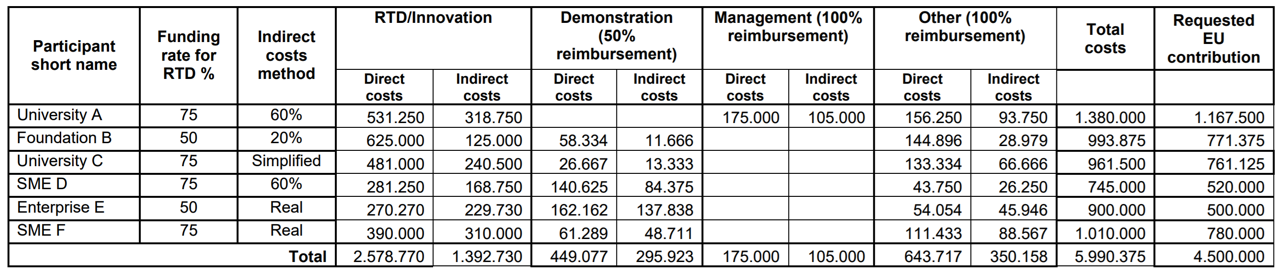
\includegraphics[scale=0.45]{./images/budget/rulesBudget2020}
\caption{Factsheet. Rules under Horizon 2020.}
\label{rules}
\end{figure}

\textbf{HIRO}

HIRO will have as main task the coordination and project management as well as part of research and innovation. For these reasons a 5\% budget allocation is decided. Of these 200.000\EUR, most of it is assigned to personnel costs and the rest to other direct costs, indirect costs and a small part to subcontracting for tasks where University department cannot work on.
 
\textbf{Airbus Defence and Space GmbH}

Airbus Defence and Space GmbH is assigned a 10\% of the overall budget, summing a total of 400.000\EUR, a very important part of it dedicated to personnel costs and another important part to other costs derived from the design, development and manufacturing of sensors, communication systems and other components.

\textbf{BHO Legal}

BHO Legal Rechtsanwälte Partnership, as part of the legal and regulatory advisers, and specialised in industry and research institutions, is assigned a 2,5\% corresponding to 100.000\EUR, of which the vast majority is for personnel expenses.

\textbf{Deimos Space S.L.U}

Deimos is together with Thales Alenia Space SAS the main industrial partner focused on design, engineering, development and manufacturing of solutions for the aerospace sector. Deimos is responsible for technology implementation in many sectors, from telecommunications to the space sector. Its involvement in many other space projects and the experience and technology available makes Deimos a relevant company for the project when it comes to development and manufacturing. For this reason a total of 1.100.000\EUR (27,5\%) is allocated, with a distribution of 385.000\EUR to other direct costs, which includes manufacturing, and the rest to personnel costs.
 
\textbf{ICUBE-SERTIT}

A university-like budget assignation has been decided according to the nature of this stakeholder and its strong links to research and development entities. Thus, a 12,5\% of the total budget estimated has been assigned to ICUBE-SERTIT; this means 500.000\EUR \ out of 4 million.

Inside ICUBE-SERTIT, given the strong scientific component of the stakeholder, the vast majority of the budget will be assigned to the direct personnel costs of the engineering department (60\%). An 8\% will be assigned to contingencies and the rest will be approximately equally assigned in between management, marketing and partnership \& networks departments. 

\textbf{ReSAC}

ReSAC is an SME based in Bulgaria that facilitates implementation and use of remote sensing applications as well as geographic information systems (GIS). Given that it is a small company, a 2,5\% of the budget has been assigned to it, a 60\% of which will be assigned to the engineering department, management and partnership \& networks will be assigned a 15\% each and the rest will be distributed in between marketing and contingencies departments. 

\textbf{Thales Alenia Space SAS}

Being Thales a multinational specialised in space and aerospace systems and thus being technologically very developed compared to other stakeholders in terms of research, manufacturing and engineering, a total of 1.400.000\EUR \ of the total budget has been assigned to it (which represents a 35\% of the total budget). 

Inside Thales departments, the heaviest weight of the budget has been assigned to the engineering department (40\% or 336.000\EUR) given the technological nature of the company. Nevertheless, relatively close behind are the management and the manufacturing departments which receive a 17,5\% of the budget each (147.000\EUR). Marketing and partnership \& networks departments get a 10\% of the budget each and contingencies department gets the rest of the total budget in terms of direct personnel costs.
 
\textbf{VITO}

VITO is a data provider and sensor researcher and developer, and thus it has been assigned a lower percentage of the budget due to the lack of manufacturing processes that carry behind the need for raw materials or factories. A 5\% of the total budget (200.000\EUR) has been assigned to it. Inside VITO’s, the majority of the budget is shared between the management and the engineering departments given the strong presence of both components in their daily operations.



\section{Project organization}

\subsection{Customers}

{The following customers are defined for this project.}
% Please add the following required packages to your document preamble:
% \usepackage[table,xcdraw]{xcolor}
% If you use beamer only pass "xcolor=table" option, i.e. \documentclass[xcolor=table]{beamer}
\begin{longtable}{ll}
	
	\toprule[2pt]
	
	\textbf{Customer group}    & \textbf{Customer representative}
	\\ \midrule[1.5pt]
	
	CGG: NPA Satellite Mapping Ltd & Jean-Georges Malcor - Chief Executive officer\\
	CloudEO AG & Dr. Manfred Krischke - Co-Founder and CEO\\
	Esri BeLux & Frederik Waûnters - Manager\\
	European Space Agency (ESA) & Lionel Hernandez - Station manager in Spain\\
	Eurosense&André Jadot - CEO\\
	Geomatrix UAB & Gedas Vaitkus - Company Manager\\
	Harris&Ed Zoiss - Electronic Systems\\
	Insar&Martin Leško - Cartography expert\\
	Noveltis&Jeff Vinuesa -Business Unit Manager\\
	SpaceBel&Bernard Plano - International business development\\
	Walphot&Yves Reginster - Account manager
	\\ \bottomrule[2pt]
	
	\caption{List of customers}
	\label{table_customers}
\end{longtable}
\subsection{Stakeholders}
The stakeholders of the project will be classified depending on its role/responsbility. The possible roles and responsibilities are shown in Table \ref{table_definicionesobvias}.


\begin{longtable}{l p{10cm}}
		
	\toprule[2pt]
		
	\textbf{Roles/Responsibilities}& \textbf{Definition } 
	\\ \midrule[1.5pt]
	\endhead
		
	Interested & Entity with interest in the project or its result without the authority to contribute in it.
	\\ \midrule

	Competitor & Entity with similar interest as the ones of the present project without authority to contribute in it but with the probability of working in the same field in other projects.
	\\ \midrule

	Consortium member & Entity interested in the project that will actively collaborate in its elaboration as a partner.
	\\ \midrule

	Customer & Entity with interest in the results of the project and with authority to request updates and propose modifications.
	\\ \midrule

	Investor & Entity that will support the project financially. It has interest in the project and the authority to request updates and propose modifications.
	\\ \bottomrule[2pt]

	\caption{Definition of roles and responsibilities of stakeholders}
	\label{table_definicionesobvias}

\end{longtable}


The key stakeholders in this project are the ones shown in Table \ref{table_stakeholders}.

\begin{small}
\begin{longtable}{p{9.5cm}l}

	\toprule[2pt]
		
	\textbf{Stakeholder Name} & \textbf{Roles/Responsibilities } 
	\\ \midrule[1.5pt]
	\endhead

	ACRI-ST SAS & Interested\\
	Agroapps PCC & Interested\\
	Air and Space Evidence & Interested\\
	Airborne technologies & Competitor\\
	Airbus Defence and Space GmbH & Consortium member  \\ 
	AnsuR Technologoes & Competitor\\
	Assimila & Interested\\
	Balam Ingeniería de Sistemas & Competitor\\
	BHO Legal Rechtsanwälte Partnership & Consortium member\\ 
	CGG: NPA Satellite Mapping Ldt&Customer\\
	CloudEO AG&Customer\\
	Deimos Space S.L.U.  & Consortium member \\
	DHI-GRAS&Potential customer\\
	Esri BeLux&Customer\\
	European Association of Remote Sensing Companies (EARSC)&Interested\\
	European Comission&Main investor and customer\\
	European Council&Regulation\\
	European Space Agency (ESA)&Customer\\ 
	Eurosense&Customer\\
	Exelis&Customer\\
	Flyby&Competitor\\
	GAF AG&Competitor\\
	GEOMATRIX UAB&Customer\\
	GEOSYSTEMS&Interested\\
	GISAT&Competitor\\
	Harris&Customer\\
	High Innovative Remote Observation (HIRO) & Consortium member \\ 
	ICUBE-SERTIT                        & Consortium member \\ 
	Insar&Customer\\
	Non-European space agencies&Competitors\\
	Noveltis&Customer\\
	Remote Sensing Application Center (ReSAC)                               & Consortium member \\
	Space applications services NV/SA&Interested\\
	SpaceBel&Customer\\
	Telspazio&Interested\\
	Thales Alenia Space SAS             & Consortium member                                                                       \\ 
	VITO nv                             & Consortium member \\
	Walphot&Customer\\

	\bottomrule[2pt]

	\caption{List of stakeholders, roles and responsibilities}
	\label{table_stakeholders}

\end{longtable}
\end{small}

\subsection{Roles and responsibilities}
The following key roles have been defined for this project:
\begin{center}
	\begin{longtable}{>{\raggedright\arraybackslash}p{3cm}>{\raggedright\arraybackslash}p{3cm}>{\raggedright\arraybackslash}p{3cm}>{\raggedright\arraybackslash}p{5cm}}
		\toprule[2pt]
		\textbf{Role} & \textbf{Resource Name} & \textbf{Organization} & \textbf{Responsabilities} \\ \midrule[1.5pt] \endhead
		Project Sponsor & Luís Manuel Pérez Llera & European Commission & Supervise the project. \\ \hline
		Project Manager & Pol Fontanes Molina & HIRO & Manage the project. \\ \hline
		Project Secretary & Sílvia González García & HIRO & Administrate the internal documents and information of the group to ensure communication between the members. \\ \hline
		Financial Manager & Santiago Lopezbarrena Arenas & HIRO & Estimate and control the costs of the project. \\ \hline
		Stakeholders \& Procurement Manager & Eva María Urbano González & HIRO & Identify the stakeholders of the project and control their engagement. Plan, conduct and control the procurements of the project.\\ \hline
		Scope \& Time Manager & Marina Pons Daza & HIRO & Define and control the scope of the project. \\ \hline
		Risk Manager & Borja Calderón Rosario & HIRO & Identify and manage the possible risks of the project. \\ \hline
		Quality Manager & Guillermo Escartín Vivancos & HIRO & Control the quality requirements of the project. \\ \hline
		Technical Managers & David Pérez Sánchez, Hamza Nachett, Laura Pla Olea & HIRO & Identify, analyse and control the technical aspects of the project. \\ \hline
		Marketing \& Communications Managers & Albert Herrando Moraira, María De Benedicto Barba & HIRO & Promote the project and its final product. Search for possible customers. Identify, analyse and control the technical aspects of the project. \\ \hline
		Research \& Development assessor & - & Airbus Defence and Space GmbH & Collaboration in the research and production of satellite sensors. \\ \hline
		Legal \& Business Assessor & - & BHO Legal Rechtsanwälte Partnership & Business and legal advice. \\ \hline
		Research \& Development Assessor & - & Deimos Space S.L.U. & Design and development of satellite sensors and systems. \\ \hline
		Application collaborator & - & ICUBE-SERTIT & Assessment in the application of data provided by EO satellites such as Sentinel. \\ \hline
		Application collaborator & - & Remote Sensing Application Center (ReSAC) & Assessment in the application of remote sensing and geographic information systems products for land cover/land use, urban planning, infrastructure, etc. \\ \hline
		Development \& Testing collaborator & - & Thales Alenia Space SAS & Design, development, integration and testing of space systems. \\ \hline
		Development \& Application collaborator & - & VITO nv & Assesment in the possible use of remote sensing for land use. Development of new remote sensing systems, sensors and platforms. \\ \bottomrule[2pt]
		\caption{Roles and responsibilities}
		\label{table_roles}	
	\end{longtable}
\end{center}

\chapter{Stakeholder identification}

\section{Stakeholder analysis matrix}
\section{Stakeholder register}

\begin{center}
	\begin{longtable}{>{\raggedright\arraybackslash}p{2.2cm} >{\raggedright\arraybackslash}p{1.5cm} >{\raggedright\arraybackslash}p{2cm} >{\raggedright\arraybackslash}p{2.2cm} >{\raggedright\arraybackslash}p{2cm} >{\raggedright\arraybackslash}p{1.4cm} >{\raggedright\arraybackslash}p{2.1cm}}
		
		\toprule[2pt]
		
		\textbf{Name} & \textbf{Role} & \textbf{Contact Information} & \textbf{Requirements} & \textbf{Expectations} & \textbf{Influence} & \textbf{Classification} \\ 
		
		\midrule[1.5pt] \endhead
		
		Airbus Defence and Space GmbH & Consortium member & \textit{+33 562194040} & Innovation in optical sensors and the development of their technology & Obtain new knowledge in optical sensors and in the technology to develop them & Manage closely & Internal/ Supporter \\ \hline
		
		High Innovative Remote Observation (HIRO) & Consortium member & \textit{+34 677261221} & Integration of new EO technologies into the Copernicus Programme & Develop the project & Manage closely & Internal/ Main participant \\ \hline
		
		BHO Legal Rechtsanwälte Partnership & Consortium member & \textit{+49 2212709560 \newline \newline cologne@bho -legal.com} & Wide legal knowledge & Legal issues management & Manage closely & Internal/ Supporter \\ \hline
		
		Deimos Space S.L.U. & Consortium member & \textit{+34 918063450 \newline \newline info@elecnor- deimos.com} & Innovation in EO technology & Develop new technology for EO & Manage closely & Internal/ Supporter \\ \hline
		
		ICUBE-SERTIT & Consortium member & \textit{+33 368854645 \newline \newline sertit@icube. unistra.fr} & Innovation in urban planning & Develop new solutions for urban planning using EO & Manage closely & Internal/ Supporter \\ \hline
		
		Remote Sensing Application Center (ReSAC) & Consortium member & \textit{+359 29800731 \newline \newline resac@techno -link.com} & Innovation in urban planning & Develop new solutions for urban planning using EO & Manage closely & Internal/ Supporter \\ \hline
		
		Thales Alenia Space SAS & Consortium member & \textit{+33 157778000} & Innovation in EO technology & Develop new technology for EO & Manage closely & Internal/ Supporter \\ \hline
		
		VITO nv & Consortium member & \textit{+32 14335511} & Innovation in optical sensors and their possible uses & Obtain new knowledge in optical sensors and develop new uses for urban planning & Manage closely & Internal/ Supporter \\ \hline
		
		European Council & Regulation & \textit{+32 22816111} & Provide the legal environment for the development of the project & Fulfil the regulations and laws & Keep informed & External/ Supporter \\ \hline
		
		European Comission & Main investor and customer & \textit{+32 22999696} & Provide funding for the project & Evaluate the viability of the project & Manage closely & Internal/ Supporter \\ \hline
		
		Esri BeLux & Customer & \textit{+32 24607480 \newline \newline info@esribelu x.com} & - & Invest in a profitable project & Keep satisfied & External/ Influencer \\ \hline
		
		European Space Agency (ESA) & Customer & \textit{+33 153697654} & - & Invest in a profitable project & Keep satisfied & External/ Influencer \\ \hline
		
		Harris & Customer & \textit{1-855-477- 4272} & - & Invest in a profitable project & Keep satisfied & External/ Influencer \\ \hline
		
		SpaceBel & Customer & \textit{+32 43618111} & - & Invest in a profitable project & Keep satisfied & External/ Influencer \\ \hline
		
		Walphot & Customer & \textit{+32 81302401 \newline \newline info@walphot. com} & - & Invest in a profitable project & Keep satisfied & External/ Influencer \\ \hline
		
		CGG: NPA Satellite Mapping Ldt & Potential customer & \textit{www.cgg.com /en/What-W e-Do/GeoCon sulting/NPA} & - & Invest in a profitable project & Keep informed & External/ Influencer \\ \hline
		
		CloudEO AG & Potential customer & \textit{+49 89206021166 \newline \newline info@cloudeo -ag.com} & - & Invest in a profitable project & Keep informed & External/ Influencer \\ \hline
		
		DHI-GRAS & Potential customer & \textit{+45 45169100 \newline \newline gras@dhigrou p.com} & - & Invest in a profitable project & Keep informed & External/ Influencer \\ \hline
		
		Eurosense & Potential customer & \textit{+32 24607000 \newline \newline info@eurosen se.com} & - & Invest in a profitable project & Keep informed & External/ Influencer \\ \hline
		
		GEOMATRIX UAB & Potential customer & \textit{www.geomat rix.lt/cms/in dex.php} & - & Invest in a profitable project & Keep informed & External/ Influencer \\ \hline
		
		Insar & Potential customer & \textit{+421 233006847 \newline \newline matusbakon @insar.sk} & - & Invest in a profitable project & Keep informed & External/ Influencer \\ \hline
		
		Noveltis & Potential customer & \textit{+33 0562881111 \newline \newline contact@nov eltis.fr} & - & Invest in a profitable project & Keep informed & External/ Influencer \\ \hline
		
		Airborne technologies & Competitor & \textit{+43 2622347182 00 \newline \newline office@airbo rnetechnolog ies.at} & - & Be a profitable project & Monitor & External/ Reluctant \\ \hline
		
		AnsuR Technologoes & Competitor & \textit{+47 64009456 \newline \newline contact@ans ur.no} & - & Failure of the project & Monitor & External/ Reluctant \\ \hline
		
		Balam Ingeniería de Sistemas & Competitor & \textit{info@balami s.com} & - & Failure of the project & Monitor & External/ Reluctant \\ \hline
		
		Flyby & Competitor & \textit{+39 0586505016 \newline \newline info@flyby.it} & - & Failure of the project & Monitor & External/ Reluctant \\ \hline
		
		GAF AG & Competitor & \textit{+49 891215280 \newline \newline info@gaf.de} & - & Failure of the project & Monitor & External/ Reluctant \\ \hline
		
		GISAT & Competitor & \textit{+42 271741935 \newline \newline gisat@gisat.cz} & - & Failure of the project & Monitor & External/ Reluctant \\ \hline
		
		Non-European space agencies & Competitors & \textit{} & - & Failure of the project & Monitor & External/ Reluctant \\ \hline
		
		ACRI-ST SAS & Interested & \textit{+33 492967500 \newline \newline information@ acri-st.fr} & - & Get interesting information about project updates & Keep informed & External/ Neutral \\ \hline
		
		Agroapps PCC & Interested & \textit{+30 2310253810 \newline \newline info@agroap ps.gr} & - & Get information about the project & Keep informed & External/ Neutral \\ \hline
		
		Air and Space Evidence & Interested & \textit{+44 7860473172} & - & Get information about the project & Keep informed & External/ Neutral \\ \hline
		
		Assimila & Interested & \textit{info@assimil a.eu} & - & Get information about the project & Keep informed & External/ Neutral \\ \hline
		
		European Association of Remote Sensing Companies (EARSC) & Interested &\textit{info@earsc.org} & - & Get information about the project & Keep informed & External/ Neutral \\ \hline
		
		GEOSYSTEMS & Interested & \textit{+48 228511166 \newline \newline office@geosy stems.pl} & - & Get information about the project & Keep informed & External/ Neutral \\ \hline
		
		Space applications services NV/SA & Interested & \textit{+32 27215484 \newline \newline info@spaceap plications.com} & - & Get information about the project & Keep informed & External/ Neutral \\ \hline
		
		Telspazio & Interested & \textit{+39 08353751 \newline \newline info@e-geos.it} & - & Get information about the project & Keep informed & External/ Neutral \\ \hline
		
		\bottomrule[2pt]
		
		\caption{Stakeholder register}
		\label{stakeholder_register}
	\end{longtable}
\end{center}








% BIBLIOGRAPHY

% styles:
%	abbrv   : [#] Initial. Surname (pages and vol. abbrev.)
% 	acm     : [#] Surname, Initial. (sc)
%	alpha   : [Abrev.yy] Name Surname
%	apalike : [Surname, yyyy] Surname, Initial 
%	ieeetr  : [#] Initial. Surname (pages and vol. ext.)
%	plain   : [#] Name Surname
%	siam    : [#] Initial. Surname (sc)
%	unsrt   : [#] Name Surname

\bibliographystyle{plain}
\bibliography{Projects_G3} 


\end{document}